\documentclass{article} % For LaTeX2e
\usepackage{iclr2020_conference,times}

% Optional math commands from https://github.com/goodfeli/dlbook_notation.
%%%%%% NEW MATH DEFINITIONS %%%%%

\usepackage{amsmath,amsfonts,bm}

% Mark sections of captions for referring to divisions of figures
\newcommand{\figleft}{{\em (Left)}}
\newcommand{\figcenter}{{\em (Center)}}
\newcommand{\figright}{{\em (Right)}}
\newcommand{\figtop}{{\em (Top)}}
\newcommand{\figbottom}{{\em (Bottom)}}
\newcommand{\captiona}{{\em (a)}}
\newcommand{\captionb}{{\em (b)}}
\newcommand{\captionc}{{\em (c)}}
\newcommand{\captiond}{{\em (d)}}

% Highlight a newly defined term
\newcommand{\newterm}[1]{{\bf #1}}


% Figure reference, lower-case.
\def\figref#1{figure~\ref{#1}}
% Figure reference, capital. For start of sentence
\def\Figref#1{Figure~\ref{#1}}
\def\twofigref#1#2{figures \ref{#1} and \ref{#2}}
\def\quadfigref#1#2#3#4{figures \ref{#1}, \ref{#2}, \ref{#3} and \ref{#4}}
% Section reference, lower-case.
\def\secref#1{section~\ref{#1}}
% Section reference, capital.
\def\Secref#1{Section~\ref{#1}}
% Reference to two sections.
\def\twosecrefs#1#2{sections \ref{#1} and \ref{#2}}
% Reference to three sections.
\def\secrefs#1#2#3{sections \ref{#1}, \ref{#2} and \ref{#3}}
% Reference to an equation, lower-case.
\def\eqref#1{equation~\ref{#1}}
% Reference to an equation, upper case
\def\Eqref#1{Equation~\ref{#1}}
% A raw reference to an equation---avoid using if possible
\def\plaineqref#1{\ref{#1}}
% Reference to a chapter, lower-case.
\def\chapref#1{chapter~\ref{#1}}
% Reference to an equation, upper case.
\def\Chapref#1{Chapter~\ref{#1}}
% Reference to a range of chapters
\def\rangechapref#1#2{chapters\ref{#1}--\ref{#2}}
% Reference to an algorithm, lower-case.
\def\algref#1{algorithm~\ref{#1}}
% Reference to an algorithm, upper case.
\def\Algref#1{Algorithm~\ref{#1}}
\def\twoalgref#1#2{algorithms \ref{#1} and \ref{#2}}
\def\Twoalgref#1#2{Algorithms \ref{#1} and \ref{#2}}
% Reference to a part, lower case
\def\partref#1{part~\ref{#1}}
% Reference to a part, upper case
\def\Partref#1{Part~\ref{#1}}
\def\twopartref#1#2{parts \ref{#1} and \ref{#2}}

\def\ceil#1{\lceil #1 \rceil}
\def\floor#1{\lfloor #1 \rfloor}
\def\1{\bm{1}}
\newcommand{\train}{\mathcal{D}}
\newcommand{\valid}{\mathcal{D_{\mathrm{valid}}}}
\newcommand{\test}{\mathcal{D_{\mathrm{test}}}}

\def\eps{{\epsilon}}


% Random variables
\def\reta{{\textnormal{$\eta$}}}
\def\ra{{\textnormal{a}}}
\def\rb{{\textnormal{b}}}
\def\rc{{\textnormal{c}}}
\def\rd{{\textnormal{d}}}
\def\re{{\textnormal{e}}}
\def\rf{{\textnormal{f}}}
\def\rg{{\textnormal{g}}}
\def\rh{{\textnormal{h}}}
\def\ri{{\textnormal{i}}}
\def\rj{{\textnormal{j}}}
\def\rk{{\textnormal{k}}}
\def\rl{{\textnormal{l}}}
% rm is already a command, just don't name any random variables m
\def\rn{{\textnormal{n}}}
\def\ro{{\textnormal{o}}}
\def\rp{{\textnormal{p}}}
\def\rq{{\textnormal{q}}}
\def\rr{{\textnormal{r}}}
\def\rs{{\textnormal{s}}}
\def\rt{{\textnormal{t}}}
\def\ru{{\textnormal{u}}}
\def\rv{{\textnormal{v}}}
\def\rw{{\textnormal{w}}}
\def\rx{{\textnormal{x}}}
\def\ry{{\textnormal{y}}}
\def\rz{{\textnormal{z}}}

% Random vectors
\def\rvepsilon{{\mathbf{\epsilon}}}
\def\rvtheta{{\mathbf{\theta}}}
\def\rva{{\mathbf{a}}}
\def\rvb{{\mathbf{b}}}
\def\rvc{{\mathbf{c}}}
\def\rvd{{\mathbf{d}}}
\def\rve{{\mathbf{e}}}
\def\rvf{{\mathbf{f}}}
\def\rvg{{\mathbf{g}}}
\def\rvh{{\mathbf{h}}}
\def\rvu{{\mathbf{i}}}
\def\rvj{{\mathbf{j}}}
\def\rvk{{\mathbf{k}}}
\def\rvl{{\mathbf{l}}}
\def\rvm{{\mathbf{m}}}
\def\rvn{{\mathbf{n}}}
\def\rvo{{\mathbf{o}}}
\def\rvp{{\mathbf{p}}}
\def\rvq{{\mathbf{q}}}
\def\rvr{{\mathbf{r}}}
\def\rvs{{\mathbf{s}}}
\def\rvt{{\mathbf{t}}}
\def\rvu{{\mathbf{u}}}
\def\rvv{{\mathbf{v}}}
\def\rvw{{\mathbf{w}}}
\def\rvx{{\mathbf{x}}}
\def\rvy{{\mathbf{y}}}
\def\rvz{{\mathbf{z}}}

% Elements of random vectors
\def\erva{{\textnormal{a}}}
\def\ervb{{\textnormal{b}}}
\def\ervc{{\textnormal{c}}}
\def\ervd{{\textnormal{d}}}
\def\erve{{\textnormal{e}}}
\def\ervf{{\textnormal{f}}}
\def\ervg{{\textnormal{g}}}
\def\ervh{{\textnormal{h}}}
\def\ervi{{\textnormal{i}}}
\def\ervj{{\textnormal{j}}}
\def\ervk{{\textnormal{k}}}
\def\ervl{{\textnormal{l}}}
\def\ervm{{\textnormal{m}}}
\def\ervn{{\textnormal{n}}}
\def\ervo{{\textnormal{o}}}
\def\ervp{{\textnormal{p}}}
\def\ervq{{\textnormal{q}}}
\def\ervr{{\textnormal{r}}}
\def\ervs{{\textnormal{s}}}
\def\ervt{{\textnormal{t}}}
\def\ervu{{\textnormal{u}}}
\def\ervv{{\textnormal{v}}}
\def\ervw{{\textnormal{w}}}
\def\ervx{{\textnormal{x}}}
\def\ervy{{\textnormal{y}}}
\def\ervz{{\textnormal{z}}}

% Random matrices
\def\rmA{{\mathbf{A}}}
\def\rmB{{\mathbf{B}}}
\def\rmC{{\mathbf{C}}}
\def\rmD{{\mathbf{D}}}
\def\rmE{{\mathbf{E}}}
\def\rmF{{\mathbf{F}}}
\def\rmG{{\mathbf{G}}}
\def\rmH{{\mathbf{H}}}
\def\rmI{{\mathbf{I}}}
\def\rmJ{{\mathbf{J}}}
\def\rmK{{\mathbf{K}}}
\def\rmL{{\mathbf{L}}}
\def\rmM{{\mathbf{M}}}
\def\rmN{{\mathbf{N}}}
\def\rmO{{\mathbf{O}}}
\def\rmP{{\mathbf{P}}}
\def\rmQ{{\mathbf{Q}}}
\def\rmR{{\mathbf{R}}}
\def\rmS{{\mathbf{S}}}
\def\rmT{{\mathbf{T}}}
\def\rmU{{\mathbf{U}}}
\def\rmV{{\mathbf{V}}}
\def\rmW{{\mathbf{W}}}
\def\rmX{{\mathbf{X}}}
\def\rmY{{\mathbf{Y}}}
\def\rmZ{{\mathbf{Z}}}

% Elements of random matrices
\def\ermA{{\textnormal{A}}}
\def\ermB{{\textnormal{B}}}
\def\ermC{{\textnormal{C}}}
\def\ermD{{\textnormal{D}}}
\def\ermE{{\textnormal{E}}}
\def\ermF{{\textnormal{F}}}
\def\ermG{{\textnormal{G}}}
\def\ermH{{\textnormal{H}}}
\def\ermI{{\textnormal{I}}}
\def\ermJ{{\textnormal{J}}}
\def\ermK{{\textnormal{K}}}
\def\ermL{{\textnormal{L}}}
\def\ermM{{\textnormal{M}}}
\def\ermN{{\textnormal{N}}}
\def\ermO{{\textnormal{O}}}
\def\ermP{{\textnormal{P}}}
\def\ermQ{{\textnormal{Q}}}
\def\ermR{{\textnormal{R}}}
\def\ermS{{\textnormal{S}}}
\def\ermT{{\textnormal{T}}}
\def\ermU{{\textnormal{U}}}
\def\ermV{{\textnormal{V}}}
\def\ermW{{\textnormal{W}}}
\def\ermX{{\textnormal{X}}}
\def\ermY{{\textnormal{Y}}}
\def\ermZ{{\textnormal{Z}}}

% Vectors
\def\vzero{{\bm{0}}}
\def\vone{{\bm{1}}}
\def\vmu{{\bm{\mu}}}
\def\vtheta{{\bm{\theta}}}
\def\va{{\bm{a}}}
\def\vb{{\bm{b}}}
\def\vc{{\bm{c}}}
\def\vd{{\bm{d}}}
\def\ve{{\bm{e}}}
\def\vf{{\bm{f}}}
\def\vg{{\bm{g}}}
\def\vh{{\bm{h}}}
\def\vi{{\bm{i}}}
\def\vj{{\bm{j}}}
\def\vk{{\bm{k}}}
\def\vl{{\bm{l}}}
\def\vm{{\bm{m}}}
\def\vn{{\bm{n}}}
\def\vo{{\bm{o}}}
\def\vp{{\bm{p}}}
\def\vq{{\bm{q}}}
\def\vr{{\bm{r}}}
\def\vs{{\bm{s}}}
\def\vt{{\bm{t}}}
\def\vu{{\bm{u}}}
\def\vv{{\bm{v}}}
\def\vw{{\bm{w}}}
\def\vx{{\bm{x}}}
\def\vy{{\bm{y}}}
\def\vz{{\bm{z}}}

% Elements of vectors
\def\evalpha{{\alpha}}
\def\evbeta{{\beta}}
\def\evepsilon{{\epsilon}}
\def\evlambda{{\lambda}}
\def\evomega{{\omega}}
\def\evmu{{\mu}}
\def\evpsi{{\psi}}
\def\evsigma{{\sigma}}
\def\evtheta{{\theta}}
\def\eva{{a}}
\def\evb{{b}}
\def\evc{{c}}
\def\evd{{d}}
\def\eve{{e}}
\def\evf{{f}}
\def\evg{{g}}
\def\evh{{h}}
\def\evi{{i}}
\def\evj{{j}}
\def\evk{{k}}
\def\evl{{l}}
\def\evm{{m}}
\def\evn{{n}}
\def\evo{{o}}
\def\evp{{p}}
\def\evq{{q}}
\def\evr{{r}}
\def\evs{{s}}
\def\evt{{t}}
\def\evu{{u}}
\def\evv{{v}}
\def\evw{{w}}
\def\evx{{x}}
\def\evy{{y}}
\def\evz{{z}}

% Matrix
\def\mA{{\bm{A}}}
\def\mB{{\bm{B}}}
\def\mC{{\bm{C}}}
\def\mD{{\bm{D}}}
\def\mE{{\bm{E}}}
\def\mF{{\bm{F}}}
\def\mG{{\bm{G}}}
\def\mH{{\bm{H}}}
\def\mI{{\bm{I}}}
\def\mJ{{\bm{J}}}
\def\mK{{\bm{K}}}
\def\mL{{\bm{L}}}
\def\mM{{\bm{M}}}
\def\mN{{\bm{N}}}
\def\mO{{\bm{O}}}
\def\mP{{\bm{P}}}
\def\mQ{{\bm{Q}}}
\def\mR{{\bm{R}}}
\def\mS{{\bm{S}}}
\def\mT{{\bm{T}}}
\def\mU{{\bm{U}}}
\def\mV{{\bm{V}}}
\def\mW{{\bm{W}}}
\def\mX{{\bm{X}}}
\def\mY{{\bm{Y}}}
\def\mZ{{\bm{Z}}}
\def\mBeta{{\bm{\beta}}}
\def\mPhi{{\bm{\Phi}}}
\def\mLambda{{\bm{\Lambda}}}
\def\mSigma{{\bm{\Sigma}}}

% Tensor
\DeclareMathAlphabet{\mathsfit}{\encodingdefault}{\sfdefault}{m}{sl}
\SetMathAlphabet{\mathsfit}{bold}{\encodingdefault}{\sfdefault}{bx}{n}
\newcommand{\tens}[1]{\bm{\mathsfit{#1}}}
\def\tA{{\tens{A}}}
\def\tB{{\tens{B}}}
\def\tC{{\tens{C}}}
\def\tD{{\tens{D}}}
\def\tE{{\tens{E}}}
\def\tF{{\tens{F}}}
\def\tG{{\tens{G}}}
\def\tH{{\tens{H}}}
\def\tI{{\tens{I}}}
\def\tJ{{\tens{J}}}
\def\tK{{\tens{K}}}
\def\tL{{\tens{L}}}
\def\tM{{\tens{M}}}
\def\tN{{\tens{N}}}
\def\tO{{\tens{O}}}
\def\tP{{\tens{P}}}
\def\tQ{{\tens{Q}}}
\def\tR{{\tens{R}}}
\def\tS{{\tens{S}}}
\def\tT{{\tens{T}}}
\def\tU{{\tens{U}}}
\def\tV{{\tens{V}}}
\def\tW{{\tens{W}}}
\def\tX{{\tens{X}}}
\def\tY{{\tens{Y}}}
\def\tZ{{\tens{Z}}}


% Graph
\def\gA{{\mathcal{A}}}
\def\gB{{\mathcal{B}}}
\def\gC{{\mathcal{C}}}
\def\gD{{\mathcal{D}}}
\def\gE{{\mathcal{E}}}
\def\gF{{\mathcal{F}}}
\def\gG{{\mathcal{G}}}
\def\gH{{\mathcal{H}}}
\def\gI{{\mathcal{I}}}
\def\gJ{{\mathcal{J}}}
\def\gK{{\mathcal{K}}}
\def\gL{{\mathcal{L}}}
\def\gM{{\mathcal{M}}}
\def\gN{{\mathcal{N}}}
\def\gO{{\mathcal{O}}}
\def\gP{{\mathcal{P}}}
\def\gQ{{\mathcal{Q}}}
\def\gR{{\mathcal{R}}}
\def\gS{{\mathcal{S}}}
\def\gT{{\mathcal{T}}}
\def\gU{{\mathcal{U}}}
\def\gV{{\mathcal{V}}}
\def\gW{{\mathcal{W}}}
\def\gX{{\mathcal{X}}}
\def\gY{{\mathcal{Y}}}
\def\gZ{{\mathcal{Z}}}

% Sets
\def\sA{{\mathbb{A}}}
\def\sB{{\mathbb{B}}}
\def\sC{{\mathbb{C}}}
\def\sD{{\mathbb{D}}}
% Don't use a set called E, because this would be the same as our symbol
% for expectation.
\def\sF{{\mathbb{F}}}
\def\sG{{\mathbb{G}}}
\def\sH{{\mathbb{H}}}
\def\sI{{\mathbb{I}}}
\def\sJ{{\mathbb{J}}}
\def\sK{{\mathbb{K}}}
\def\sL{{\mathbb{L}}}
\def\sM{{\mathbb{M}}}
\def\sN{{\mathbb{N}}}
\def\sO{{\mathbb{O}}}
\def\sP{{\mathbb{P}}}
\def\sQ{{\mathbb{Q}}}
\def\sR{{\mathbb{R}}}
\def\sS{{\mathbb{S}}}
\def\sT{{\mathbb{T}}}
\def\sU{{\mathbb{U}}}
\def\sV{{\mathbb{V}}}
\def\sW{{\mathbb{W}}}
\def\sX{{\mathbb{X}}}
\def\sY{{\mathbb{Y}}}
\def\sZ{{\mathbb{Z}}}

% Entries of a matrix
\def\emLambda{{\Lambda}}
\def\emA{{A}}
\def\emB{{B}}
\def\emC{{C}}
\def\emD{{D}}
\def\emE{{E}}
\def\emF{{F}}
\def\emG{{G}}
\def\emH{{H}}
\def\emI{{I}}
\def\emJ{{J}}
\def\emK{{K}}
\def\emL{{L}}
\def\emM{{M}}
\def\emN{{N}}
\def\emO{{O}}
\def\emP{{P}}
\def\emQ{{Q}}
\def\emR{{R}}
\def\emS{{S}}
\def\emT{{T}}
\def\emU{{U}}
\def\emV{{V}}
\def\emW{{W}}
\def\emX{{X}}
\def\emY{{Y}}
\def\emZ{{Z}}
\def\emSigma{{\Sigma}}

% entries of a tensor
% Same font as tensor, without \bm wrapper
\newcommand{\etens}[1]{\mathsfit{#1}}
\def\etLambda{{\etens{\Lambda}}}
\def\etA{{\etens{A}}}
\def\etB{{\etens{B}}}
\def\etC{{\etens{C}}}
\def\etD{{\etens{D}}}
\def\etE{{\etens{E}}}
\def\etF{{\etens{F}}}
\def\etG{{\etens{G}}}
\def\etH{{\etens{H}}}
\def\etI{{\etens{I}}}
\def\etJ{{\etens{J}}}
\def\etK{{\etens{K}}}
\def\etL{{\etens{L}}}
\def\etM{{\etens{M}}}
\def\etN{{\etens{N}}}
\def\etO{{\etens{O}}}
\def\etP{{\etens{P}}}
\def\etQ{{\etens{Q}}}
\def\etR{{\etens{R}}}
\def\etS{{\etens{S}}}
\def\etT{{\etens{T}}}
\def\etU{{\etens{U}}}
\def\etV{{\etens{V}}}
\def\etW{{\etens{W}}}
\def\etX{{\etens{X}}}
\def\etY{{\etens{Y}}}
\def\etZ{{\etens{Z}}}

% The true underlying data generating distribution
\newcommand{\pdata}{p_{\rm{data}}}
% The empirical distribution defined by the training set
\newcommand{\ptrain}{\hat{p}_{\rm{data}}}
\newcommand{\Ptrain}{\hat{P}_{\rm{data}}}
% The model distribution
\newcommand{\pmodel}{p_{\rm{model}}}
\newcommand{\Pmodel}{P_{\rm{model}}}
\newcommand{\ptildemodel}{\tilde{p}_{\rm{model}}}
% Stochastic autoencoder distributions
\newcommand{\pencode}{p_{\rm{encoder}}}
\newcommand{\pdecode}{p_{\rm{decoder}}}
\newcommand{\precons}{p_{\rm{reconstruct}}}

\newcommand{\laplace}{\mathrm{Laplace}} % Laplace distribution

\newcommand{\E}{\mathbb{E}}
\newcommand{\Ls}{\mathcal{L}}
\newcommand{\R}{\mathbb{R}}
\newcommand{\emp}{\tilde{p}}
\newcommand{\lr}{\alpha}
\newcommand{\reg}{\lambda}
\newcommand{\rect}{\mathrm{rectifier}}
\newcommand{\softmax}{\mathrm{softmax}}
\newcommand{\sigmoid}{\sigma}
\newcommand{\softplus}{\zeta}
\newcommand{\KL}{D_{\mathrm{KL}}}
\newcommand{\Var}{\mathrm{Var}}
\newcommand{\standarderror}{\mathrm{SE}}
\newcommand{\Cov}{\mathrm{Cov}}
% Wolfram Mathworld says $L^2$ is for function spaces and $\ell^2$ is for vectors
% But then they seem to use $L^2$ for vectors throughout the site, and so does
% wikipedia.
\newcommand{\normlzero}{L^0}
\newcommand{\normlone}{L^1}
\newcommand{\normltwo}{L^2}
\newcommand{\normlp}{L^p}
\newcommand{\normmax}{L^\infty}

\newcommand{\parents}{Pa} % See usage in notation.tex. Chosen to match Daphne's book.

\DeclareMathOperator*{\argmax}{arg\,max}
\DeclareMathOperator*{\argmin}{arg\,min}

\DeclareMathOperator{\sign}{sign}
\DeclareMathOperator{\Tr}{Tr}
\let\ab\allowbreak

\usepackage{amsmath,amsfonts,bm}

\usepackage{hyperref}
\usepackage{url}
\usepackage{breqn}
\usepackage{booktabs}
\usepackage{siunitx} % used in SHREC table
\usepackage{bbm}        % for mathbbm
\usepackage{graphicx} \graphicspath{{figures/}}
\usepackage[export]{adjustbox} % figure vertical alignment
%\usepackage{floatrow} % figure and table together
\usepackage{capt-of} % or \usepackage{caption} % figure and table together
\usepackage{subfig}
%\usepackage{wrapfig}
%\usepackage{floatflt}
\usepackage{amsthm}
\usepackage{amsmath}
\usepackage{amssymb}
\usepackage{wrapfig}

%\title{Which spherical CNN should you use?\\ DeepSphere V2}
\title{DeepSphere: a graph-based spherical CNN}
%\title{DeepSphere: an efficient graph-based spherical CNN}
%\title{DeepSphere, an efficient (& equivariant) graph-based spherical CNN}

\author{Michaël Defferrard, Martino Milani \& Frédérick Gusset \\
Institute of Electrical Engineering, EPFL, Lausanne, Switzerland \\
\texttt{\{michael.defferrard,martino.milani,frederick.gusset\}@epfl.ch}
\AND
Nathanaël Perraudin \\
Swiss Data Science Center (SDSC), Zurich, Switzerland \\
\texttt{nathanael.perraudin@sdsc.ethz.ch}
}

\newtheorem{definition}{Definition}[section]
\newtheorem{theorem}{Theorem}[section]
\newtheorem{prop}{Proposition}
\newtheorem*{remark}{Remark}
\newcommand{\norm}[1]{\left\lVert#1\right\rVert}
\renewcommand{\b}[1]{{\bm{#1}}}  % bold symbol
\newcommand{\bO}{\mathcal{O}}
\newcommand{\R}{\mathbb{R}}
\renewcommand{\S}{\mathbb{S}}
\newcommand{\G}{\mathcal{G}}  % graph
\newcommand{\V}{\mathcal{V}}  % vertex set
\newcommand{\E}{\mathcal{E}}  % edge set
\DeclareMathOperator*{\diag}{diag}

\newcommand{\fix}{\marginpar{FIX}}
\newcommand{\new}{\marginpar{NEW}}
\newcommand{\todo}[1]{{\color[rgb]{.6,.1,.6}{#1}}}
\newcommand{\nati}[1]{{\color[rgb]{.3,.5,.9}{#1}}}
\newcommand{\mart}[1]{{\color[rgb]{.9,.5,.3}{#1}}}

\newcommand{\figref}[1]{figure~\ref{fig:#1}}
\newcommand{\Figref}[1]{Figure~\ref{fig:#1}}
\newcommand{\tabref}[1]{table~\ref{tab:#1}}
\newcommand{\Tabref}[1]{Table~\ref{tab:#1}}
\newcommand{\secref}[1]{section~\ref{sec:#1}}
\newcommand{\Secref}[1]{Section~\ref{sec:#1}}
%\newcommand{\secref}[1]{\S\ref{sec:#1}}
\newcommand{\eqnref}[1]{equation~(\ref{eqn:#1})}
\newcommand{\Eqnref}[1]{Equation~(\ref{eqn:#1})}

\newcommand{\linefrac}[2]{
    {#1/#2}
}

%\iclrfinalcopy % Uncomment for camera-ready version, but NOT for submission.
\begin{document}

\begin{description}
	\item[git] \url{https://github.com/nperraud/deepsphere_v2_paper}
	\item[overleaf] \url{https://www.overleaf.com/project/5d31d2fbd6859d54cb707212}
\end{description}

story: there are tradeoffs when designing a spherical CNN -> DS strikes a controllable balance between efficiency / cost and exactitude / equivariance
% DSv2 has a clear tradeoff between equivariance and computational cost

* method development: tool that solve a need (balance btw the desiderata: equiv vs cost)\\
* research question: anisotropy (highlight from the start or leave it as a dangling question in the end)\\

contributions:\\
* theory $\Rightarrow$ convergence (better graph)\\
* experiments on relevant problems (not spherical MNIST) $\Rightarrow$ check the desiderata\\
  * surprising: anisotropy doesn't seem useful\\

\todo{
\begin{itemize}
	\item shall we really name it? Or simply reference the general idea of a graph-based spherical CNN.
	\item adjacency matrix: $A$ instead of $W$?
	\item anonymize DeepSphere citation
% 	\item climate spherical figure: inputs with TC and AR labels superimposed [Frédérick]
	\item citet for inline, citep for parenthesis
	\item More details on related work? Not sure we have the space. If yes, detailed comparison with related work after method.
	\item PSD of climate data: how does it compare to cosmo and 3D objects?
	\item align the spheres in figure 1
	\item mention that \citep{esteves2018sphericalcnn} and \citep{cohen2018sphericalcnn} computed equivariance error
	\item check footnotes
	\item climate data on spectrum plot
	\item result tables: only what supports the main message in the text, everything we have in the appendix
	\item Unify vocabulary. Sampling, discretization, or pixelization of the sphere? Signal, maps, functions. Irregular, uneven. Coarsening, down-sampling.
	\item check English vs American English
	\item unify enumerations. I like (i), (ii), etc.
	\item notation: should we use indices from 1 to n instead of 0 to n-1 for compactness?
	\item add \citet{bruna2013gnn} in equivariance? They were the first to do a spherical CNN with graphs. Graph is built from a uniform random sampling of the sphere.
	\item figure placements
	\item do the experiments on the icosahedral grid with the pooling as defined in the paper
	\item put all the code (learning experiments from Frédérick and equivariance experiments from Martino) in a common reproducible git repository to be linked from the paper
	\item update pygsp and merge sphere branch
	\item check that NN architectures and hyper-params are correctly reported
	\item keep NN architecture and hyper-params in the main text? Move the paragraph to appendix if not enough space.
	%\item shall we still site adam and batch norm? no, mainstream enough
	\item check results for ModelNet40 and integrate in text
	\item Check that HEALPix is introduced in the introduction
	\item heuristic used to set the kernel width in v1. Add values to \figref{kernel_widths} for comparison.
	\item check experiments section [Frédérick]: all the results numbers and NN + training details
	\item compute the invariance error of the whole NNs (before and after training, invariance can be learned)
	\item add it with equivariance error of the convolution to \tabref{cosmo}
\end{itemize}
}
\newpage

\maketitle

\begin{abstract}
Selecting the right convolution for a spherical neural network is a delicate tradeoff between its efficiency and its exactictude with respect of equivariance. DeepSphere, as a graph based method strikes as a controllable balance between these two aspects. This contribution 1) studies empirically and theoretically how the construction of its underlying graph affects equivariance, and 2) evaluates its performance on a large set of relevant problems.
Comparison with previous work on shape classification and climate event detection suggests that anisotropic filters are an unnecessary price to pay.
% memory, computations, implementation complexity
\end{abstract}

\section{Introduction}

Spherical data is found in many applications.
% spherical data f: S^2 -> R, projection from R^3
Planetary data (such as meteorological or geological measurements) and brain activity are example of intrinsically spherical data.
The observation of the universe, LIDAR scans, and the digitalization of 3D objects are examples of projections due to observation.
See \figref{examples}.
In many applications, labels or variables are to be inferred from spherical data.
Examples are the inference of cosmological parameters from the distribution of mass in the universe \citep{perraudin2019deepspherecosmo}, the segmentation of omnidirectional images \citep{khasanova2017sphericalcnn}, and the segmentation of cyclones from Earth observation \citep{mudigonda2017climateevents}.

\begin{figure}[h]
	\centering
	\subfloat[]{
		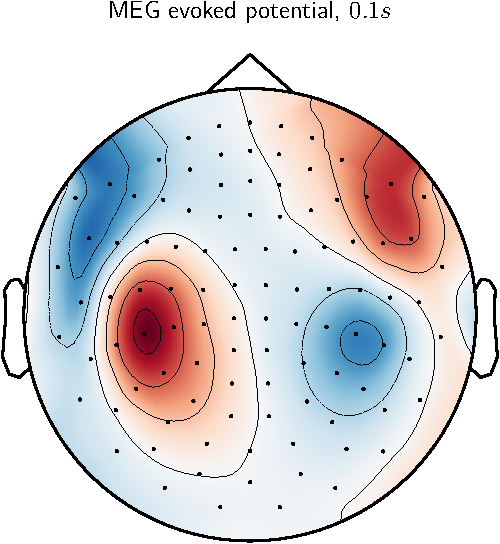
\includegraphics[height=0.20\linewidth,valign=t]{example_brain_meg}
	} \hspace{0.1em}
	\subfloat[]{
		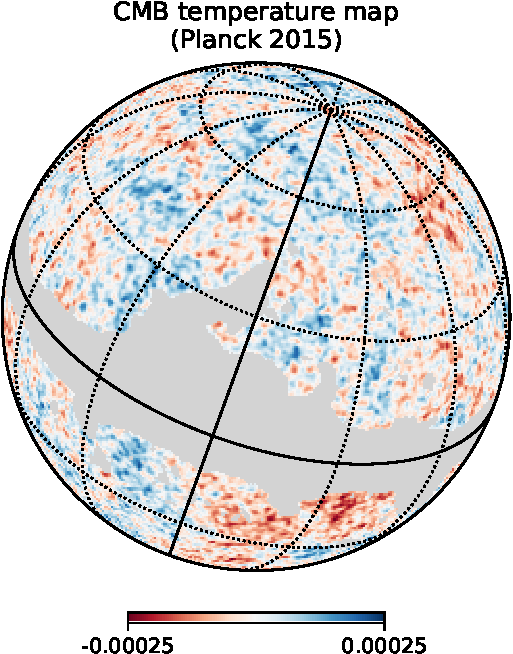
\includegraphics[height=0.20\linewidth,valign=t]{example_cosmo_cmb}
	} \hfill
	\subfloat[]{
		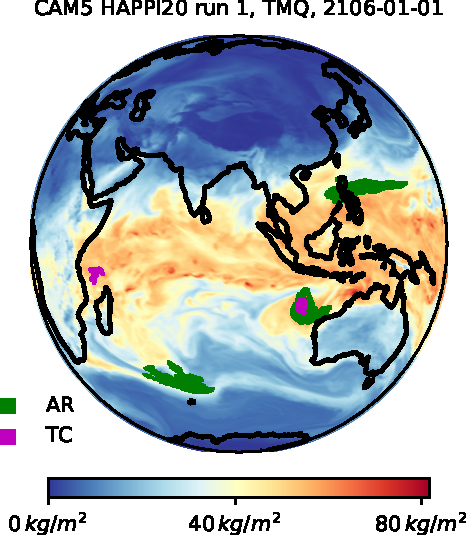
\includegraphics[height=0.20\linewidth,valign=t]{example_climate_TMQ}
		\label{fig:examples:climate}
	} \hfill
	\subfloat[]{
		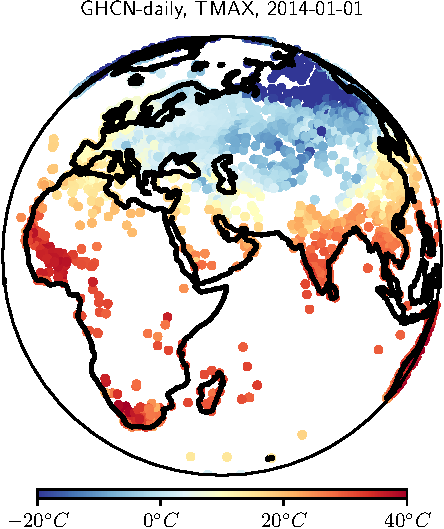
\includegraphics[height=0.20\linewidth,valign=t]{example_ghcn_daily_tmax}
		\label{fig:examples:ghcn:tmax}
	} \hfill
	\subfloat[]{
		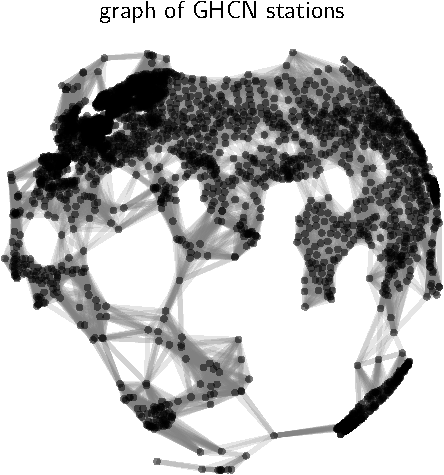
\includegraphics[height=0.20\linewidth,valign=t]{example_ghcn_graph}
		\label{fig:examples:ghcn:graph}
	}
	\caption{
		Examples of intrinsically spherical data:
		(a) brain activity recorded through magnetoencephalography (MEG),\protect\footnotemark
		(b) the cosmic microwave background (CMB) temperature from \citet{planck2015overview},
		(c) hourly precipitation from a climate simulation \citep{jiang2019sphericalcnn}, %\citep{mudigonda2017climateevents},
		(d) daily maximum temperature from the Global Historical Climatology Network (GHCN).\protect\footnotemark
		A rigid full-sphere pixelization is not ideal: brain activity is only measured on the scalp, the Milky Way's galactic plane masks observations, climate scientists desire a variable resolution, and the position of weather stations is arbitrary and changes over time.
		(e) Graphs can faithfully and efficiently represent sampled spherical data by placing vertices where data has been measured.
		%\todo{something from climate, weather?}
		%\todo{compare ideal full-spheres (like SHREC'17 projection from Esteves, 360 from Coors) to real-world measurements?}
		%\todo{horizontal colorbar for brain}
	}
	\label{fig:examples}
\end{figure}
\footnotetext[1]{\scriptsize\url{https://martinos.org/mne/stable/auto_tutorials/plot_visualize_evoked.html}}
\footnotetext[2]{\scriptsize\url{https://www.ncdc.noaa.gov/ghcn-daily-description}}

% balance of ??
% Exploit the geometrical properties of the domain, symmetries.
% desiderata or tradeoff
% We identified the following desiderata for a spherical NN.
%Those take different tradeoffs among the following desiderata.
%\begin{enumerate}
%	\item \textbf{Respect the geometry.}  % geometry, domain
%		By respecting the domain, a spherical NN should respect the symmetries of the sphere, i.e., be equivariant to rotation, and not deform the sphere, e.g., by a projection on the icosahedron.
%	\item \textbf{Generality.} % powerful
%		How general the NN is as a function approximator.
%		For example, isotropic filters are less general than anisotropic filters.
%	\item \textbf{Scalability.}
%		How a spherical CNN scales w.r.t.\ the number of pixels in terms of computational cost and memory usage.
%		% memory: feature maps and parameters
%	\item \textbf{Flexibility.}
%		Whether the NN is constrained to work on specific samplings, part of the sphere (useful when data is masked), and irregular samplings.
%	\item \textbf{Simplicity.}
%		Simplicity of its derivation and implementation.
%\end{enumerate}

% keep the story simple and focus on the tradeoff between cost (time / computational and storage / memory) and exactitude
As neural networks (NNs) have proved to be great tools for inference, variants have been developed to handle spherical data.
Exploiting the locally Euclidean property of the sphere, early attempts used standard 2D convolutions on a grid discretization of the sphere \citep{boomsma2017sphericalcnn, su2017sphericalcnn, coors2018sphericalcnn}.
While simple and efficient, those convolutions are not equivariant to rotations.
On the other side of this tradeoff, \citet{cohen2018sphericalcnn} and \citet{esteves2018sphericalcnn} proposed to perform proper spherical convolutions through the spherical harmonic transform.
While equivariant to rotations, those convolutions are expensive.

% On the one side, we have Cohen which is computationally very expensive but perfectly equivariant most general, on the other we have cube sphere which computationl very good but not equivariant at all. Other methods are tradedoff between these two. What is a good tradeoff? We think that DeepSphere is.

As the lack of equivariance penalizes performance (\secref{exp:cosmo}) and expensive convolutions prohibit their application to some real-world problems, methods standing between those two extremes are desired.
\citet{cohen2019gauge} proposed to reduce costs by limiting the size of the representation of the symmetry group.
% (from the continuous rotation group SO(3) to a discrete rotation group)
% the dimensionality of feature maps is equal to the size of the irreducible representation of the symmetry group
%As a platonic solid, it \todo{exhibits discrete rotations}.
% the representation of its symmetry group is much smaller than SO(3)
\todo{not all rotations, subset of SO(3)?}
The projection of the data from the sphere to the icosahedron however introduces distortions that might hinder performance (see the experiments in \secref{exp:climate}).
\todo{Where does Jiang fit? Need a global coordinate system (ok for planets, not projections like cosmo)}

Another approach represents the discretized sphere as a graph connecting pixels according to the distance between them \citep{bruna2013gnn, khasanova2017sphericalcnn, perraudin2019deepspherecosmo}.
While Laplacian-based graph convolutions are more efficient than spherical convolutions, they are not exactly equivariant \citep{defferrard2019deepsphereequiv}.
In this work, we argue that graph-based spherical CNNs strike an interesting balance, with a controllable tradeoff between cost and equivariance.
Experiments on multiple problems of practical interest show the competitiveness and flexibility of this approach.
% Furthermore, experiments show that, perhaps surprisingly and contrarily to previously published results \citep{cohen2019gauge} \todo{[Bronstein?]}, anisotropic filters might be an unnecessary price to pay.
% This paper focuses on improving the rotation equivariance of \citet{perraudin2019deepspherecosmo}, a scalable graph-based method designed for cosmological applications.

\section{Method}

% \begin{figure}
% 	\centering
% 	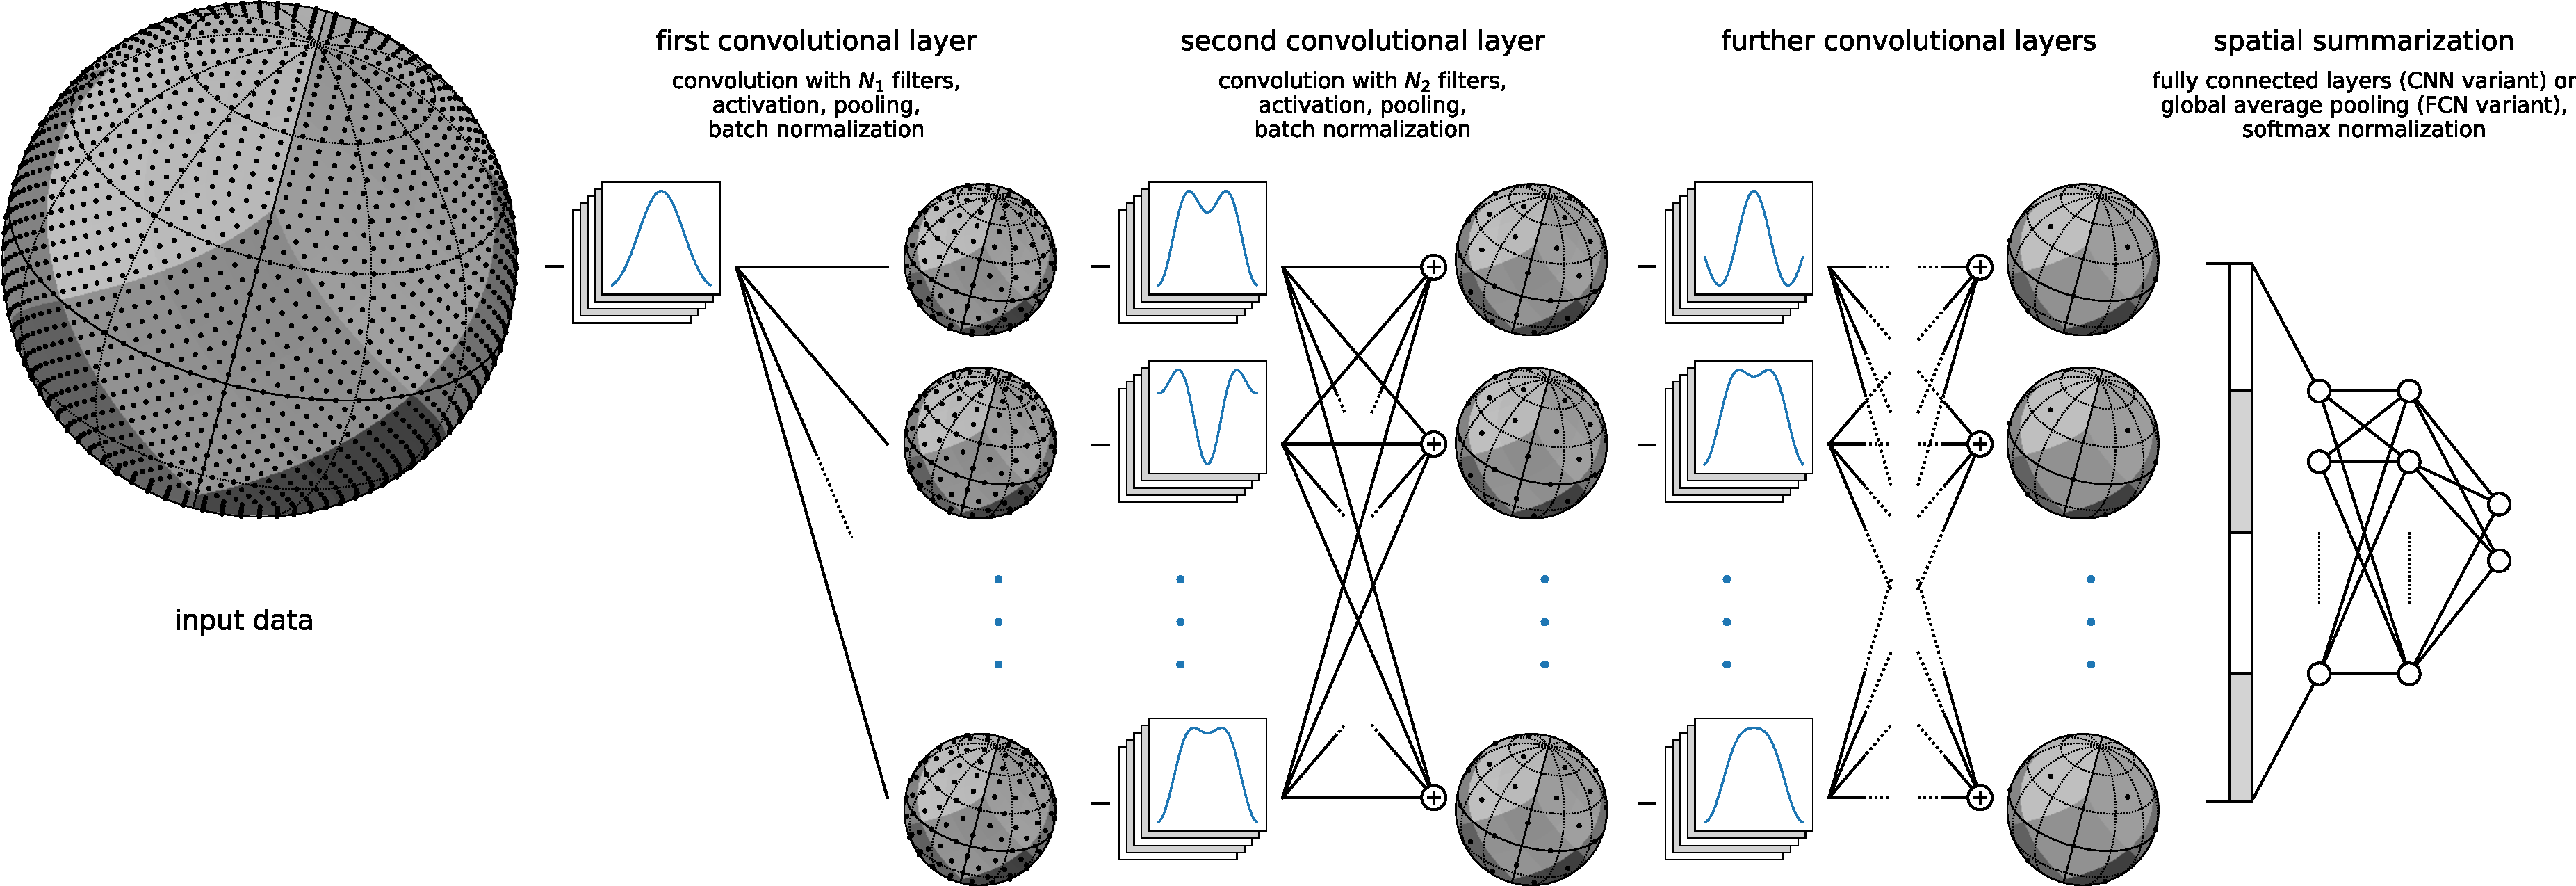
\includegraphics[width=\linewidth]{figure_architecture_v3}
% 	\caption{Example architecture from \cite{perraudin2019deepspherecosmo}.
% 		Global tasks need a spatial summarization: the FCN variant is rotation invariant (and accepts inputs of varying sizes), while the CNN variant is not.
% 		Dense tasks (when the output lives on the sphere, like segmentation) are rotation equivariant.
% 		\todo{Shall we keep this figure? It's very nice, but we could save space. ML people probably have this in mind.}
% 	}
% 	\label{fig:architecture}
% \end{figure}

DeepSphere leverages graph convolutions to achieve the following properties: (i) computational efficiency, (ii) sampling flexibility, and (iii) rotation equivariance (\secref{equivariance}).
% An example architecture is shown in \figref{architecture}.
The main idea is to model the discretized sphere as a graph of connected pixels: the length of the shortest path between two pixels is an approximation of the geodesic distance between them.
We use the graph CNN formulation introduced in \citep{defferrard2016graphnn} and a pooling strategy that exploits hierarchical pixelizations of the sphere.

\paragraph{Sampling.}
Given a sampling scheme $\V = \{x_i \in \S^2\}_{i=1}^n$, a function $f : \S^2 \supset F_\V \to \R$ is sampled as $T_\V(f) = \b{f}$ by the sampling operator $T_\V: L^2(\S^2) \supset F_\V \to \R^n$ defined as $\b{f}: f_i=f(x_i)$, where $F_\V$ will be specified in \secref{equivariance}.
As there is no analogue of uniform sampling on the sphere, many schemes have been proposed with different tradeoffs.
In this work, depending on the considered application, we will use the equiangular \citep{driscoll1994Fouriersphere}, HEALPix \citep{gorski2005healpix}, and icosahedral \citep{baumgardner1985icosahedral} grids.

\paragraph{Graph.}
From $\V$, we construct a weighted undirected graph $\G = (\V, w)$, where the elements of $\V$ are the vertices and the weight $w_{ij} = w_{ji}$ is a similarity measure between vertices $x_i$ and $x_j$.
The combinatorial graph Laplacian $\b{L} \in \R^{n \times n}$ is defined as $\b{L} = \b{D} - \b{A}$, where $\b{A} = (w_{ij})$ is the weighted adjacency matrix, $\b{D} = (d_{ii})$ is the diagonal degree matrix, and $d_{ii} = \sum_j w_{ij}$ is the weighted degree of vertex $x_i$.
%$\b{D} = \diag(\b{A} \b{1})$
Given a sampling scheme $\V$, usually fixed by the application or the available measurements, the freedom in constructing $\G$ is in setting $w$.
\Secref{equivariance} shows how to set $w$ to minimize the equivariance error.
%building a good graph amounts to set a good $w$.

\paragraph{Convolution.}
On Euclidean domains, convolutions are efficiently implemented by sliding a window in the signal domain.
On the sphere however, there is no straightforward way to implement a convolution in the signal domain due to non-uniform samplings.
Convolutions are most often performed in the spectral domain through a spherical harmonic transform (SHT).
That is the approach taken by \citet{cohen2018sphericalcnn} and \citet{esteves2018sphericalcnn}, which has a computational cost of $\bO(n^{3/2})$ on isolatitude pixelizations (such as the HEALPix and equiangular grids) and $\bO(n^2)$ in general.
On the other hand, following \citet{defferrard2016graphnn}, graph convolutions can be defined as
\begin{equation} \label{eqn:graph_conv}
	h(\b{L}) \b{f} = \left(\sum_{i=0}^K \alpha_i \b{L}^i\right) \b{f},
\end{equation}
where $K$ is the polynomial order (which corresponds to the filter's size) and $\alpha_i$ are the coefficients to be optimized during training.\footnote{In practice, training with Chebyshev polynomials (instead of monomials) is slightly more stable. We believe it to be due to their orthogonality and uniformity.}
Those convolutions are used by \citet{khasanova2017sphericalcnn} and \citet{perraudin2019deepspherecosmo} and cost $\bO(n)$ operations through a recursive application of $\b{L}$.\footnote{As long as the graph is sparsified such that the number of edges, i.e., the number of non-zeros in $\b{A}$, is proportional to the number of vertices $n$. This can always be done as most weights are very small.}

\paragraph{Pooling.}
Down- and up-sampling is natural for hierarchical pixelizations,\footnote{The equiangular, HEALPix, and icosahedral schemes are of this kind.} where each subdivision divides a pixel in (an equal number of) child sub-pixels.
To pool (down-sample), the data supported on the sub-pixels is summarized by a permutation invariant function such as the maximum or the average.
To unpool (up-sample), the data supported on a pixel is copied to all its sub-pixels.
% Frédérick: Dans le cas de l'icosahedron, le pooling n'est pas invariant à la permutation (on prend la valeur du 1er pixel, sans regarder les autres)
% Frédérick: Et le unpooling est correct uniquement dans le cas de l'average pooling (mais on fait pas de max pooling dans ce cas). Encore une fois, l'icosahedron est inspiré de Jiang, où 1 seul sub-pixel prend la valeur du pixel, le reste est rempli avec des '1'

\paragraph{Architecture.}
All our NNs are fully convolutional, and employ a global average pooling (GAP) for rotation invariant tasks.
Graph convolutional layers are always followed by batch normalization and ReLU activation, except in the last layer.
Note that batch normalization and activation act on the elements of $\b{f}$ independently, and hence don't depend on the domain of $f$.
%We denote graph convolutional layers with $C$ output channels as $GC_C$ and fully connected layers with $C$ output neurons as $FC_C$.
%Those linear layers are always followed by batch normalization and ReLU activation, except in the last layer.
%softmax normalization as $SM$
%Pooling and unpooling by a factor $F$ are denoted as $P_F$ and $P^{-1}_F$, global average pooling as $GAP$.

% \section{Notation}
% Throughout this contribution, we denote with bold font all vectors and matrices such as $\b{L}$ the graph Laplacian and $\b{f}$ the vector of the sampled function $f$.
% \nati{Right now, it is not True}
% % , a weighted undirected graph $G(V, E, \mathbf W)$,
% \nati{I do not think we should have a notation section, but should somehow write this somewhere...}
% mdeff: I think this convention is clear enough when reading.

\section{Graph convolution and equivariance} \label{sec:equivariance}
%\section{Is graph convolution equivariant to rotation? [2 pages]} \label{sec:equivariance}

While the graph framework offers great flexibility, its ability to faithfully represent the underlying sphere --- for graph convolutions to be rotation equivariant --- highly depends on the sampling locations and the graph construction.

\subsection{Problem formulation}
% 0.1 Explain the sampling problem
%As the graph convolution acts on a sampled version of the function $\b{f}$ and the rotation on its continuous counterpart $f$, a sampling operator is needed.

We require $F_\V$ to be a suitable subspace of $L^2(\S^2)$ such that $T_\V$ is invertible, i.e., the function $f \in F_\V$ can be unambiguously reconstructed from its sampled values $\b{f}$.
The existence of such a subspace depends on the sampling scheme $\V$, and its characterization is a common problem in signal processing \citep{driscoll1994Fouriersphere}.
For most sampling schemes, it is not known if $F_\V$ exists and hence if $T_\V$ is invertible.
A special case is the equiangular sampling scheme where a sampling theorem holds, and thus a closed form of $T_\V^{-1}$ is known. % \cite{driscoll1994Fouriersphere}
For sampling schemes where no such sampling formula is available, we leverage the discrete SHT to reconstruct $f$ from $\b{f}=T_\V f$, thus approximating $T_\V^{-1}$.
For all theoretical considerations, we assume that $F_\V$ exists and $f \in F_\V$.

% 0.2 Explain why the Laplacian is so important...
By definition, the (spherical) graph convolution is rotation equivariant, if and only if, it commutes with the rotation operator defined as $R(g), g\in SO(3)$: $R(g) f(x) = f\left(g^{-1} x \right)$.
In the context of this work, graph convolution is performed by recursive applications of the graph Laplacian (\eqnref{graph_conv}).
Hence, if $\b{L}$ commutes with the rotation operator, then, by recursion, it will also commute with the convolution $h(\b{L})$.
As a result, to simplify our analysis, we concentrate on the graph Laplacian and $h(\b{L})$ is rotational invariant if and only if
% 0.3 Formulate the problem
\begin{equation} \label{eq:equivariance}
	\b{R}_\V(g) \b{L} \b{f} = \b{L} \b{R}_\V(g) \b{f} \hspace{1cm} \forall f\in F_\V \text{ and } \forall g\in SO(3),
\end{equation}
where $\b{R}_\V(g) = T_\V R(g) T_\V^{-1}$. For practical a evaluation of the equivariance, we define the \textit{normalized equivariance error} for a signal $\b{f}$, and a  rotation $g$ as:
\begin{equation} \label{eq:equivariance error}
	E_{\b{L}}(\b{f}, g) = \left(\frac{ \norm {\b{R}_\V(g) \b{L} \b{f} - \b{L} \b{R}_\V(g) \b{f}} }{\norm {\b{L} \b{f}}}\right)^2,
\end{equation}
More generally for a class of signal $f \in C \subset F_\V$, the \textit{mean equivariance error} defined as
\begin{equation} \label{eq:mean equivariance error}
	\overline E_{\b{L}, C} = \mathbb E_{\b{f}\in C, g\in SO(3)} \ E_{\b{L}}(\b{f}, g),
\end{equation}
represents well the overall equivariance error.
In practice, we analyse this error with respect of the frequency by setting the set $C$ to functions $f$ made of single degree spherical harmonic.
The expected value is obtained by averaging over a finite number of random functions and random rotations.

\subsection{Finding the optimal set of weights}  \label{sec:optimal}
% 1) summary the work of Khasanova
Naturally, \cite{khasanova2017sphericalcnn} designed a Laplacian $\b{L}$ that minimizes \eqref{eq:equivariance error} for specific rotations on the longitude and latitude axis. 
Working specifically with the equiangular sampling, they consider the set $\mathcal{G}$ of all the possible graphs where each node is connected only to four of its nearest neighbours (North, South, West, East).
% and propose a weighting scheme $w_{ij}$ that minimizes \eqref{eq:equivariance error} for specific rotations on the longitude latitude axis.
Their approach leads to weights $w_{ij}$ inversely proportional to the Euclidean distance between vertices:
\begin{equation} \label{eqn:weights:khasanova}
	w_{ij} = \frac{1}{\norm{x_i-x_j}}
\end{equation}

% 2) explain our approach
We chose a different approach and take inspiration from \cite{belkin2005towards}, which proves that for a random \emph{uniform sampling} scheme the graph Laplacian converges toward the Laplace-Beltrami operator $\Delta_{\mathbb{S}^2}$ as the number of sampling points goes to infinity.
This convergence result is important as a) $\Delta_{\mathbb{S}^2}$ commutes with rotation ($\Delta_{\mathbb{S}^2}R(g) = R(g)\Delta_{\mathbb{S}^2}$) and b) is diagonalized by the spherical harmonics.
In this case the weighting scheme is full (every node is connected to every node) and is based on the exponential kernel:
\begin{equation} \label{eqn:weights:belkin}
w_{ij} = e^{-\frac{1}{4t} \norm{x_i-x_j}^2}
\end{equation}
In practice, because of the exponential, most of the weights are very close to $0$. Hence, to optimize for computational efficiency, we limit ourselves to only the $k$ nearest neighbors.
Given $k$, the optimal $t$ is found by searching for the minimizer of \eqref{eq:mean equivariance error}.
\Figref{kernel_widths} shows the optimal kernel widths found for various resolutions of the HEALPix grid.


\subsection{Analysis of the proposed weighting scheme}
We analyse our proposed weighting scheme both theoretically and empirically.

\paragraph{Theoretical convergence.}
We extend the work of Belkin and Nyiogi to a sufficiently regular, deterministic sampling scheme.
Given a sampling scheme $\V = \{x_0, \dots, x_{n-1}\}$, define $\sigma_i$ to be the patch of the surface of the sphere corresponding to $x_i$, $A_i$ its corresponding area and $d_i$ the radius of the smallest ball in $\R^3$ containing $\sigma_i$. Define $d^{(n)} := \max_{i=0, \dots, n}d_i$ and $A^{(n)}=\max_{i=0, \dots, n}A_i$.
\begin{theorem}
	For a sampling $\V = \{x_i\in\S^2\}_{i=0}^{n-1}$ of the sphere that is equi-area and such that $d^{(n)} \leq \frac{C}{\sqrt{n}}$, for all $f: \S^2 \rightarrow \R$ Lipschitz with respect to the Euclidean distance in $\R^3$, for all $y\in\S^2$, there exists a sequence $t_n = n^\beta$ such that 
% 	the rescaled Heat Kernel Graph Laplacian $\frac{|\S^2|}{4\pi t_n^2}\b {L}^t_n$ converges pointwise to the Laplace Beltrami operator on the sphere $\Delta{\S^2}$  
	\begin{equation*}
	 \lim_{n\to\infty} \frac{|\mathbb{S}^2|}{4\pi t_n^2} \b{L}_n^{t_n} T_\V f [i] =  \Delta_{\mathbb{S}^2}f(x_i)\quad \forall i=0, ..., n-1.
	\end{equation*} 
% 	for $n\to\infty$.
	\label{theo:pointwise convergence for a regular sampling}
\end{theorem}
As a direct implication of this theorem, $\b{L}$ converges pointwisely toward the Laplace-Beltrami operator ($\Delta_{\S^2}$). This operator commutes with rotation and hence this convergence is a strong hint for equivariance.
Importantly, the proof of Theorem \ref{theo:pointwise convergence for a regular sampling} in Appendix \ref{sec: appendix: proof of theorem} inspires us in the construction of our graph Laplacian. It is inspirational for the graph construction and for how the parameter $t$ needs to be adjusted with respect to the number of points $n$.

Nevetheless, it is important to keep in mind the limits of Theorem \ref{theo:pointwise convergence for a regular sampling}.
First, it is \emph{not} a proof of equivariance of the graph convolution for a specific sampling. To construct such a proof, a stronger convergence result is needed, for example uniform convergence (instead of pointwise).
% \todo{Can we intuitively write what pointwise convergence means, and how it is more limited than spectral or uniform convergence?}
We note that in the random sampling case, the graph laplacian does \emph{not} converges uniformly in general \cite{belkin2007convergence}[Sec 3], but does for a class of Lipschitz functions \cite{belkin2005towards}[Sec 6].  Second, while do not have a proof for it, we strongly believe that the HEALPix sampling does satisfy the hypothesis $d^{(n)}\leq \frac{C}{\sqrt{n}}$ of Theorem \ref{theo:pointwise convergence for a regular sampling}. The empirical results discussed in the next paragraph also point in this direction. This is further discussed in Appendix \ref{sec: appendix: proof of theorem}.


% 3) Show experimental results
\paragraph{Empirical convergence.}

% 3.0) explain how we obtained the figures
We calculated numerically the equivariance error $\bar{E}_{\b L,C(\ell)}$ \eqref{eq:mean equivariance error} as a function of the frequency (degree) $\ell$ of monochromatic signals $C(\ell)$, for different parameter sets of DeepSphere and for the graph of Khasanova and Frossard too. Results are in figure \ref{fig:equivariance_error}.
The frequencies $\ell$ of the monochromatic signals were chosen in the range $(0,\  3N_{side}-1)$ for the Healpix sampling, and in the range $(0, b)$ for the equiangular sampling, to allow for an almost perfect synthesis of the sampled signals, and thus an almost perfect implementation (up to numerical errors) of the operator $\b{R}_\V$ in equation \eqref{eq:mean equivariance error} \citep{gorski1999healpixprimer}. In this way all the error measured is due to imperfections in the empirical approximation of the Laplace-Beltrami operator.

% 3.1) explain what the figures tell us
By fixing the number of neighbors to 8, we already observe a first improvement compared to the previous version of DeepSphere, whose graph also was constructed to have at maximum 8 neighbors. By increasing the number of neighbors of the graph the equivariance error decreases by more than one order of magnitude. On the other side, by increasing the graph resolution ($N_{side}$) the equivariance error in the high frequencies decreases. The filtering operation with the graph Laplacian of Khasanova, Frossard is by construction perfectly equivariant to rotations along the vertical axis, and is designed to minimize the filtering error of vertical displacements of the same image. While these characteristics are designed for well analysing omnidirectional images, that are naturally aligned on the north-south axis, if tested on random rotations this construction shows its limits: increasing the graph resolution does not seem to improve its equivariance.


\begin{figure}
	\begin{minipage}{0.65\linewidth}
		\centering
		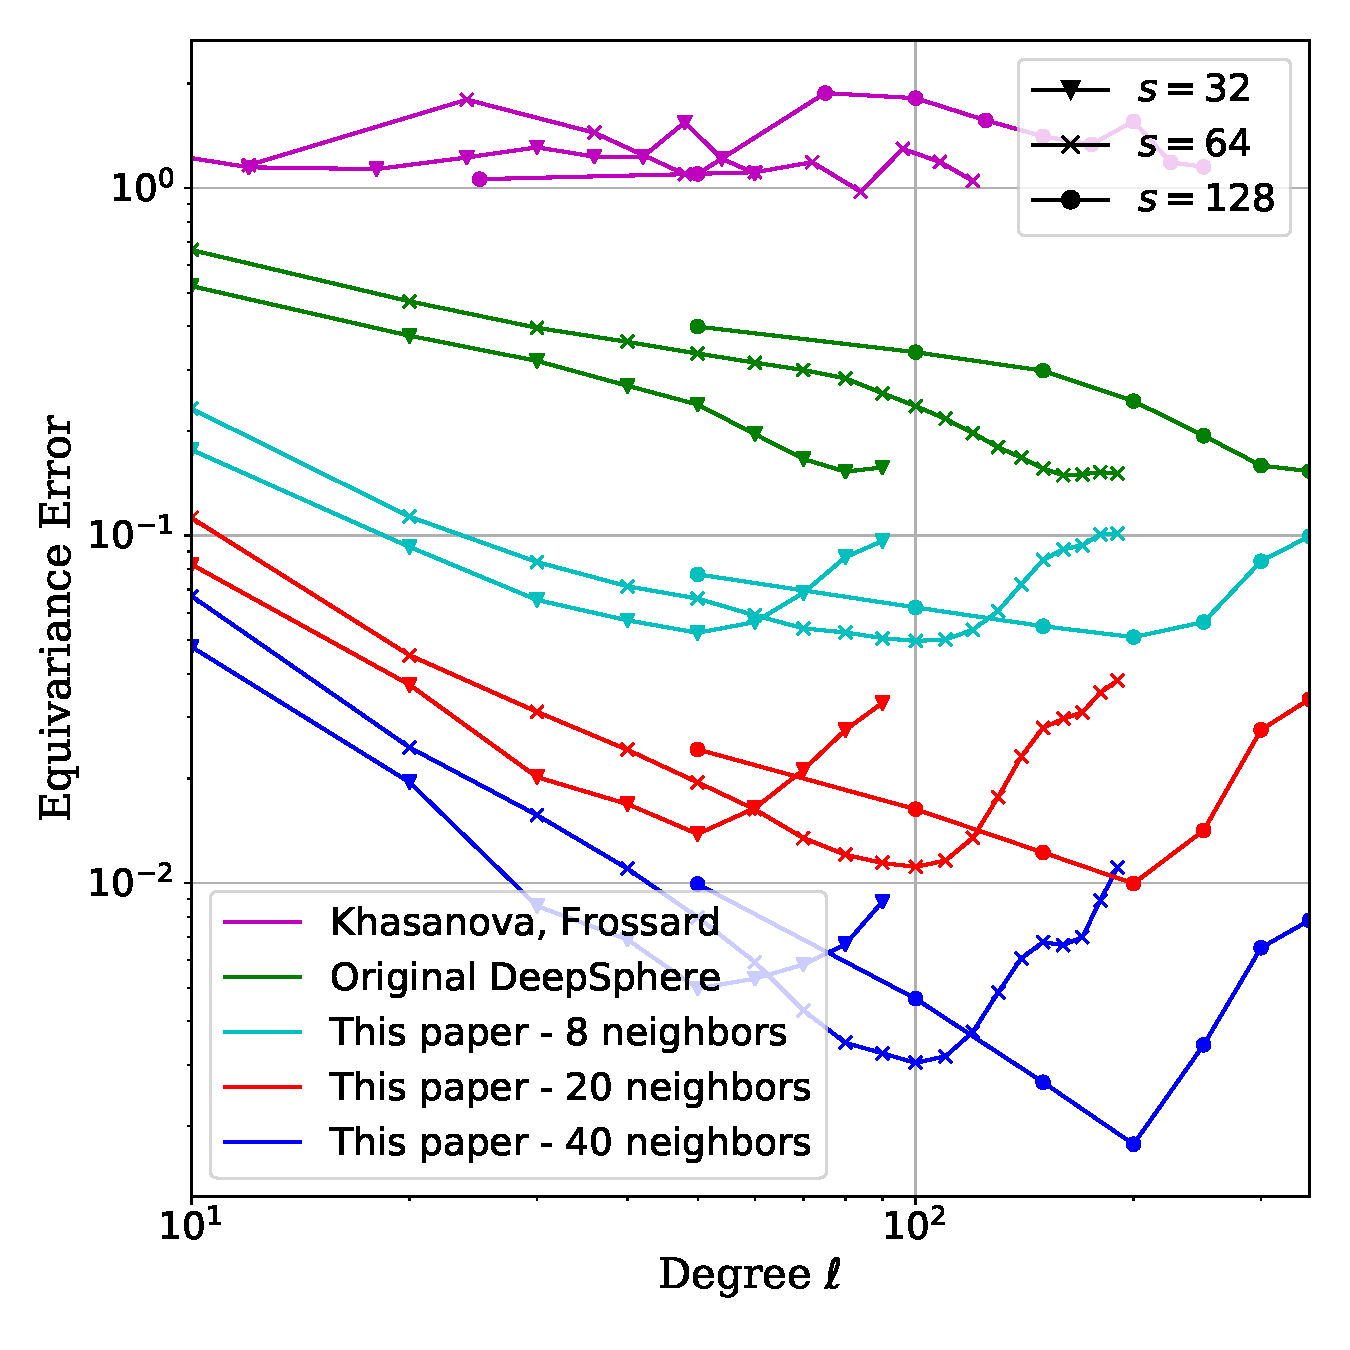
\includegraphics[width=0.9\linewidth]{all_in_one.pdf}
		\caption{Normalized mean equivariance error \eqref{eq:mean equivariance error}. The number of pixels is $4s^2$ for the equiangular sampling and $12s^2$ for the Healpix sampling.}
		\label{fig:equivariance_error}
	\end{minipage}
	\hfill
	\begin{minipage}{0.35\linewidth}
		\centering
		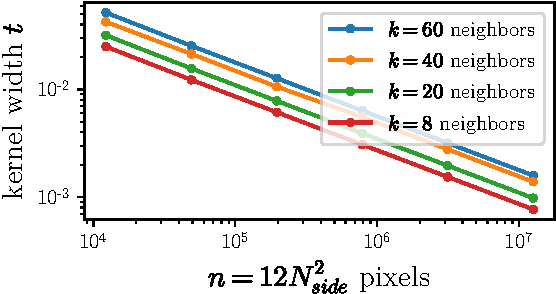
\includegraphics[width=\linewidth]{kernel_widths}
		\caption{Optimal kernel widths.}
		\label{fig:kernel_widths}
		\vspace{1em}
		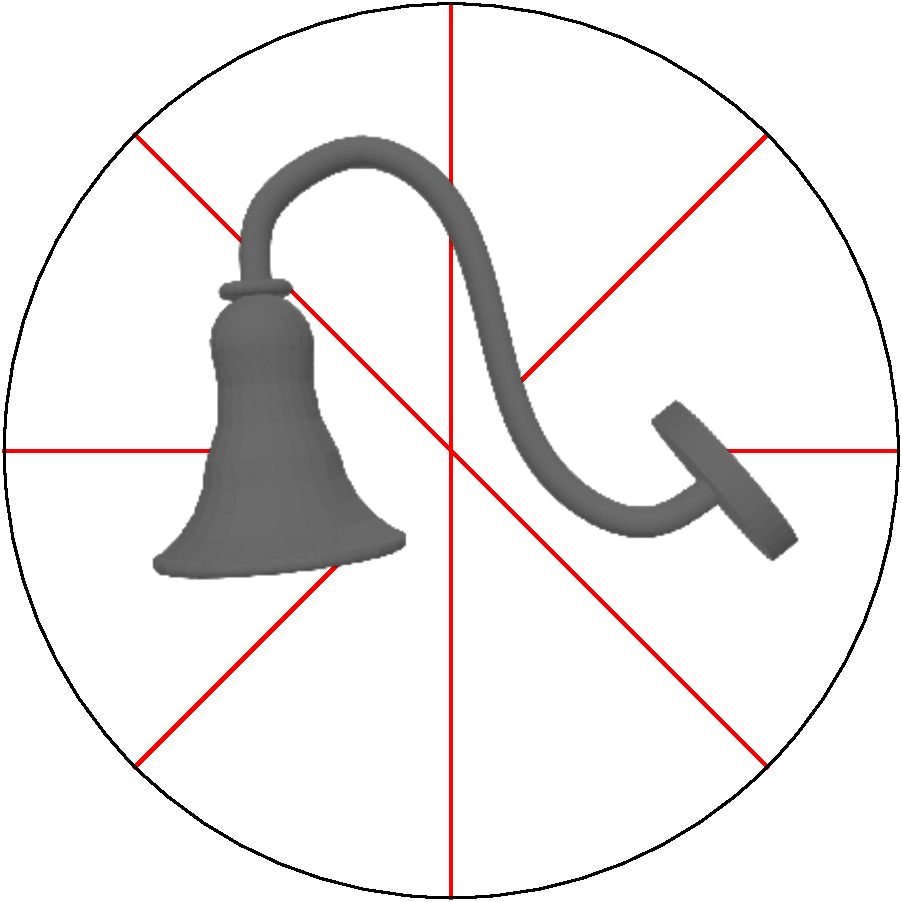
\includegraphics[height=4.5em]{lamp_000018}
		\hfill
		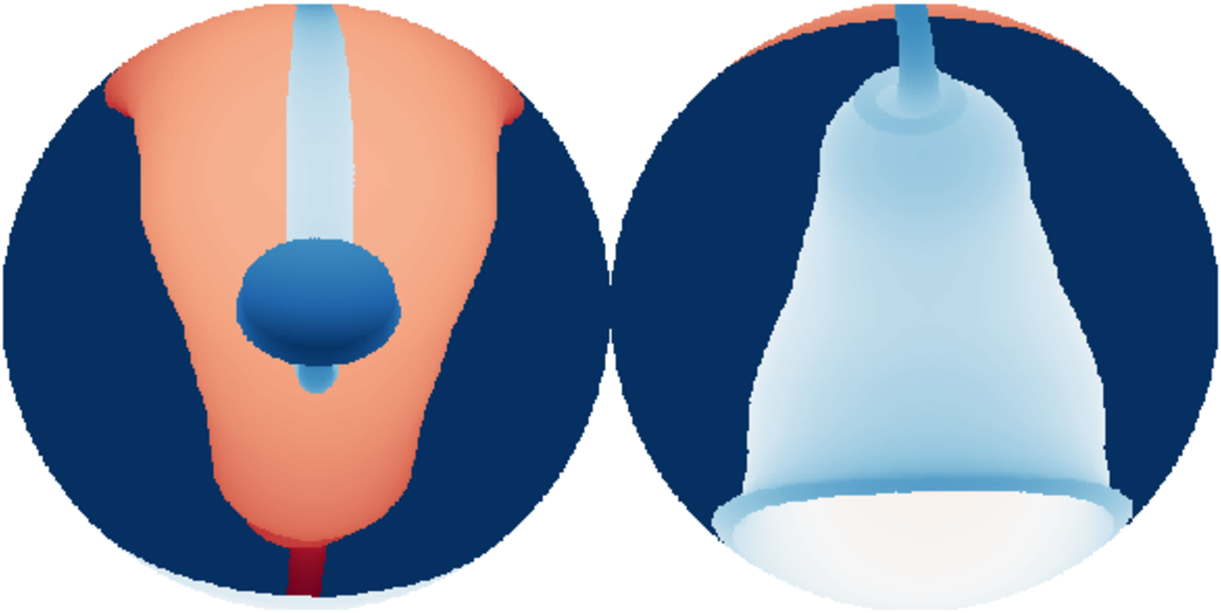
\includegraphics[height=4.5em]{lamp_000018_sphere_nobar}
		\caption{3D object represented as a spherical depth map.}
		\label{fig:depthmap}
		\vspace{1em}
		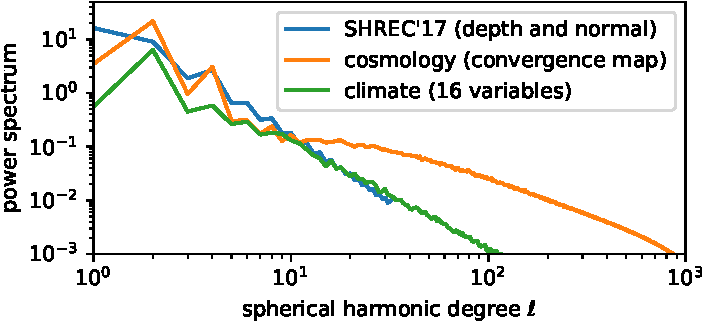
\includegraphics[width=\linewidth]{spectrum}
		\caption{Power spectral densities.}
		\label{fig:spectrum}
	\end{minipage}
\end{figure}

\section{Experiments}

% Show:
% * meet the desiderata: scale
% * DeepSphere V1 and V2 are equivalent in practice: better equivariance doesn't translate to better performance
% * anisotropy doesn't help

\subsection{3D objects recognition} \label{sec:exp:objects}

The recognition of 3D shapes is a rotation invariant task: rotating an object doesn't change its nature.
While 3D shapes are usually represented as meshes or point clouds, representing them as spherical maps (\figref{depthmap}) naturally allows a rotation invariant treatment.
%LIDAR is an example of a physical sensor that acquires spherical depth maps
%, which are a posteriori represented as point clouds.
% but there is gravity, might not really be SO(3) invariant
%\todo{move to intro?} no, good to motivate each task

The SHREC'17 shape retrieval contest \citep{shrec17} contains 51,300 randomly oriented 3D models from ShapeNet \citep{shapenet}, to be classified in 55 categories (tables, lamps, airplanes, etc.).
As in \citet{cohen2018sphericalcnn}, objects are represented by 6 spherical maps.
At each pixel, a ray is traced towards the center of the sphere.
The distance from the sphere to the object forms a depth map.
The $\cos$ and $\sin$ of the surface angle forms two normal maps.
The same is done for the object's convex hull.\footnote{Albeit we didn't observe much improvement by using the convex hull.}
The maps are discretized using either an equiangular grid with bandwidth $b = 64$ ($n = 4 b^2 = 16,384$ pixels) or an HEALPix grid with $N_{side} = 32$ ($n = 12 N_{side}^2 = 12,288$ pixels).

The equiangular graph is built with \eqnref{weights:khasanova} and $k = 4$ neighbors \citep[following][]{khasanova2017sphericalcnn}.
The HEALPix graph is built with \eqnref{weights:belkin}, $k = 8$, and a kernel width $t$ set to the average of the distances \citep[following][]{perraudin2019deepspherecosmo}.
The NN is made of $5$ graph convolutional layers, each followed by a max pooling layer which down-samples by $4$.
A GAP and a fully connected layer with softmax follow.
The polynomials are all of order $K=3$ and the number of channels per layer is $16, 32, 64, 128, 256$, respectively.
Following \citet{esteves2018sphericalcnn}, the cross-entropy plus a triplet loss is optimized with Adam for 30 epochs on the dataset augmented by 3 random translations.
The learning rate is $5 \cdot 10^{-2}$ and the batch size is 32.

\begin{table}
    \centering
	%\begin{tabular}{l cc r rr}
	\begin{tabular}{l cc r rS[table-format=2.0]}
		\toprule
		& \multicolumn{2}{c}{performance} & \multicolumn{1}{c}{size} & \multicolumn{2}{c}{speed} \\
		\cmidrule(lr){2-3} \cmidrule(lr){4-4} \cmidrule(lr){5-6}
		& F1 & mAP & params & \multicolumn{1}{c}{inference} & \multicolumn{1}{c}{training} \\
		\midrule
		% $SO(3)$ vs $S^2$ vs graph
		\citet{cohen2018sphericalcnn} ($b=128$) & - & 67.6 & 1400\,k & 38.0\,ms & 50\,h \\
		\citet{cohen2018sphericalcnn} (simplified,\protect\footnotemark $b=64$) & 78.9 & 66.5 & 400\,k & 12.0\,ms & 32\,h \\
		\citet{esteves2018sphericalcnn} ($b=64$) & 79.4 & 68.5 & 500\,k & 9.8\,ms & 3\,h \\
		DeepSphere (equiangular $b=64$) & 79.4 & 66.5 & 190\,k & 0.9\,ms & 50\,m \\
		DeepSphere (HEALPix $N_{side}=32$) & 80.7 & 68.6 & 190\,k & 0.9\,ms & 50\,m \\
		\bottomrule
	\end{tabular}
    \caption{
		Results on SHREC'17 (3D shapes). DeepSphere achieves similar performance at a much lower cost, suggesting that anisotropic filters are an unnecessary price to pay.
		% F1-score computed with sklearn, mAP from the official script of the competition.
		% inference speed = time for a single instance to do a single training pass
		% training speed = time for the neural net to train to peak performance
	}
    \label{tab:shrec17}
\end{table}
\footnotetext[5]{As implemented in \url{https://github.com/jonas-koehler/s2cnn}.}

Results are shown in \tabref{shrec17}.
As the network is trained for shape classification rather than retrieval, we report the classification F1 alongside the mAP used in the retrieval contest.\footnote{We omit the F1 for \citet{cohen2018sphericalcnn} as we didn't get the mAP reported in the paper when running it.}
DeepSphere achieves the same performance as \citet{cohen2018sphericalcnn} and \citet{esteves2018sphericalcnn} at a much lower cost, suggesting that anisotropic filters are an unnecessary price to pay.
% x times faster
As the information in those spherical maps resides in the low frequencies (\figref{spectrum}), reducing the equivariance error didn't translate into improved performance.
For the same reason, using the more uniform HEALPix discretization or lowering the resolution down to $N_{side} = 8$ ($n=768$ pixels) didn't impact performance either.
%\todo{The same conclusions are drawn from ModelNet40 (\tabref{modelnet40}).}

% Limited by representation of data? yep, treat them as point clouds

\subsection{Cosmological model classification} \label{sec:exp:cosmo}

Given observations, cosmologists estimate the posterior probability of cosmological parameters, such as the matter density $\Omega_m$ and the normalization of the matter power spectrum $\sigma_8$.
Those parameters are typically estimated by likelihood-free inference, which requires a function to predict the parameters from simulations.
% such as Approximate Bayesian computation (ABC)
As that is complicated to setup, prediction methods are typically benchmarked on the classification of spherical maps instead \citep{schmelze2017cosmologicalmodel}.
We used the same task, data, and setup as \citet{perraudin2019deepspherecosmo}: the classification of $720$ partial convergence maps made of $n \approx 10^6$ pixels ($1/12 \approx 8\%$ of a sphere at $N_{side} = 1024$) from two $\Lambda$CDM cosmological models, ($\Omega_m = 0.31$, $\sigma_8 = 0.82)$ and ($\Omega_m = 0.26$, $\sigma_8 = 0.91)$, at a relative noise level of $3.5$ (i.e., the signal is hidden in noise of $3.5$ times higher standard deviation).
% 60 maps * 12 parts = 720 parts
Convergence maps represent the distribution of over- and under-densities of mass in the universe \citep[see][for a review of gravitational lensing]{bartelman2010gravitationallensing}.

Graphs are built with \eqnref{weights:belkin}, $k = 8, 20, 40$ neighbors, and the corresponding optimal kernel widths $t$ given in \secref{optimal}.
Following \citet{perraudin2019deepspherecosmo}, the NN is made of $5$ graph convolutional layers, each followed by a max pooling layer which down-samples by $4$.
A GAP and a fully connected layer with softmax follow.
The polynomials are all of order $K=4$ and the number of channels per layer is $16, 32, 64, 64, 64$, respectively.
The cross-entropy loss is optimized with Adam for 80 epochs.
The learning rate is $2 \cdot 10^{-4} \cdot 0.999^{\textrm{step}}$ and the batch size is 8.

\begin{table}
	\begin{minipage}[b]{0.7\linewidth}
    \centering
    \begin{tabular}{l c c}
		\toprule
		& accuracy & time \\ % & training time & NN inv. error
		\midrule
		\citet{perraudin2019deepspherecosmo}, 2D CNN baseline & 54.2 & 104\,ms \\
		\citet{perraudin2019deepspherecosmo}, CNN variant, $k=8$ & 62.1 & 185\,ms \\ % & 1\,h\,45
		\citet{perraudin2019deepspherecosmo}, FCN variant, $k=8$ & 83.8 & 185\,ms \\ % & 1\,h\,45
		$k=8$  neighbors, $t$ from \secref{optimal} & 87.1 & 185\,ms \\ % & 1\,h\,45
		$k=20$ neighbors, $t$ from \secref{optimal} & 91.3 & 250\,ms \\ % & 2\,h\,30
		$k=40$ neighbors, $t$ from \secref{optimal} & 92.5 & 363\,ms \\ % & 3\,h\,45
		\bottomrule
    \end{tabular}
	\caption{
		Results on the classification of partial convergence maps.
		Lower equivariance error translates to higher performance.
	} \label{tab:cosmo}
	\end{minipage} \hfill
	\begin{minipage}[b]{0.25\linewidth}
		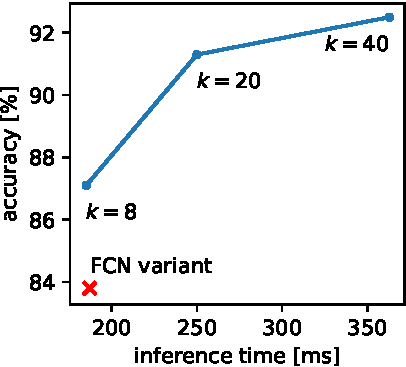
\includegraphics[width=\linewidth]{cosmo_cost_accuracy_tradeoff}
		\captionof{figure}{Tradeoff between cost and accuracy.}
		\label{fig:cosmo:tradeoff}
	\end{minipage}
\end{table}

Unlike on SHREC'17, results (\tabref{cosmo}) show that a lower equivariance error on the convolutions translates to higher performance.
That is probably due to the high frequency content of those maps (\figref{spectrum}).
There is a clear cost-accuracy tradeoff, controlled by the number of neighbors $k$ (\figref{cosmo:tradeoff}).
This experiment moreover demonstrates DeepSphere's flexibility (using partial spherical maps) and scalability (competing spherical CNNs were tested on maps of at most $10,000$ pixels).

\subsection{Climate event segmentation} \label{sec:exp:climate}

We evaluate our method on a task proposed by \citep{mudigonda2017climateevents}: the segmentation of extreme climate events, Tropical Cyclones (TC) and Atmospheric Rivers (AR), in global climate simulations (\figref{examples:climate}).
The data was produced by a 20-year run of the Community Atmospheric Model v5 (CAM5) and consists of 16 channels such as temperature, wind, humidity, and pressure at multiple altitudes.
We used the pre-processed dataset from \citep{jiang2019sphericalcnn}.\footnote{Available at \url{http://island.me.berkeley.edu/ugscnn/data}.}
%\url{https://github.com/maxjiang93/ugscnn}
%\url{https://github.com/maxjiang93/ugscnn/blob/master/experiments/exp4_sphere_climate/run.sh}
%\url{http://island.me.berkeley.edu/ugscnn/data/climate_sphere_l5.zip}
There is 1,072,805 spherical maps, down-sampled to a level-5 icosahedral grid ($n = 10 \cdot 4^l + 2 = 10,242$ pixels).
The labels are heavily unbalanced with 0.1\% TC, 2.2\% AR, and 97.7\% background (BG) pixels.

The graph is built with \eqnref{weights:belkin}, $k = 6$ neighbors, and a kernel width $t$ set to the average of the distances.
Following \citet{jiang2019sphericalcnn}, the NN is an encoder-decoder with skip connections.
Details in \secref{climate:appendix}.
%The encoder is made of $5$ graph convolutional layers, each followed by a \todo{pick-one?} pooling layer which down-samples by $4$.
%the number of channels per layer is $16, 32, 64, 64, 64$, respectively.
%The decoder is made of
The polynomials are all of order $K=3$.
The cross-entropy loss (weighted or non-weighted) is optimized with Adam for 30 epochs.
The learning rate is $1 \cdot 10{-3}$ and the batch size is 64.

\begin{table}
	\centering
	\begin{tabular}{l l l}
	\toprule
	& accuracy & mAP \\
	\midrule
	%\cite{jiang2019sphericalcnn} (paper) & 94.67 & - \\
	\cite{jiang2019sphericalcnn} (rerun) & 94.95 & 38.41 \\
	\cite{cohen2019gauge} (S2R) & 97.5 & 68.6 \\
	\cite{cohen2019gauge} (R2R) & 97.7 & 75.9 \\
	DeepSphere (weighted loss) & $97.8\pm 0.3$ & $77.15\pm 1.94$ \\
	DeepSphere (non-weighted loss) & $87.8\pm 0.5$ & $89.16\pm 1.37$ \\
	\bottomrule
	\end{tabular}
	\caption{
		Results on climate event segmentation: mean accuracy (over TC, AR, BG) and mean average precision (over TC and AR).
		DeepSphere achieves state-of-the-art performance. %, suggesting again that anisotropic filters are not necessary.
	}
	\label{tab:climate}
\end{table}

Results are shown in \tabref{climate} (details in tables~\ref{tab:climate:accuracy}, \ref{tab:climate:map} and~\ref{tab:climate:speed}).
The mean and standard deviation are computed over 5 runs.
Note that while \citet{jiang2019sphericalcnn} and \citet{cohen2019gauge} use a weighted cross-entropy loss, that is a suboptimal proxy for the mAP metric.
DeepSphere achieves state-of-the-art performance, suggesting again that anisotropic filters are unnecessary.
Note that results from \citet{mudigonda2017climateevents} cannot be directly compared as they don't use the same input channels.

Compared to \citet{cohen2019gauge}'s conclusion, it is surprising that S2R does worse than DeepSphere (which is limited to S2S).
Potential explanations are (i) that their icosahedral projection introduces harmful distortions, or (ii) that a larger architecture can compensate for the lack of generality. % powerfulness?
We indeed observed that more feature maps and depth led to higher performance (\secref{climate:appendix}).

\subsection{Uneven sampling} \label{sec:exp:ghcn}
% time series modeling? GHCN?
% Weather prediction? But it's not a real task. Rather a demo.

To demonstrate the flexibility of modeling the discretized sphere by a graph, we collected historical measurements from $n \approx 10,000$ weather stations scattered across the Earth.\footnote{\url{https://www.ncdc.noaa.gov/ghcn-daily-description}}
The spherical data is heavily non-uniformly sampled, with a much higher density of weather stations over North America than the Pacific (\figref{examples:ghcn:tmax}).
For illustration, we devised two artificial tasks.
A dense regression: predict the temperature on a given day knowing the temperature on the previous 5 days.
A global regression: predict the day (represented as one period of a sine over the year) from temperature or precipitations.
Predicting from temperature is much easier as it has a clear yearly pattern.

The graph is built with \eqnref{weights:belkin}, $k = 5$ neighbors, and a kernel width $t$ set to the average of the distances.
The equivariance property of the resulting graph has not been tested, and we don't expect it to be good due to the heavily non-uniform sampling.
The NN is made of $3$ graph convolutional layers.
The polynomials are all of order $K=0$ or $4$ and the number of channels per layer is $50, 100, 100$, respectively.
For the global regression, a GAP and a fully connected layer follow.
For the dense regression, a graph convolutional layer follows instead.
The MSE loss is optimized with RMSprop for 250 epochs.
The learning rate is $1 \cdot 10^{-3}$ and the batch size is 64.

\begin{table}
    \centering
    \begin{tabular}{
			c
			S[table-format=2.2]
			S[table-format=1.2]
			S[table-format=1.3]
			S[table-format=1.2]
			S[table-format=1.2]
			S[table-format=1.3]
			S[table-format=1.2]
			S[table-format=1.2]
			S[table-format=-1.3]
		}
		\toprule
		& \multicolumn{3}{c}{temp. (from past temp.)} & \multicolumn{3}{c}{day (from temperature)} & \multicolumn{3}{c}{day (from precipitations)} \\
		\cmidrule(lr){2-4} \cmidrule(lr){5-7} \cmidrule(lr){8-10}
		order $K$ & {MSE} & {MAE} & {R2} & {MSE} & {MAE} & {R2} & {MSE} & {MAE} & {R2} \\
		\midrule
		$0$ & 10.88 & 2.42 & 0.896 & 0.10 & 0.10 & 0.882 & 0.58 & 0.42 & -0.980 \\
		%%$1$ &  8.91 & 2.20 & 0.906 & - & - & - & - & - & - \\
		$4$ &  8.20 & 2.11 & 0.919 & 0.05 & 0.05 & 0.969 & 0.50 & 0.18 &  0.597 \\
		%$9$ &  8.38 & 2.12 & 0.915 & - & - & - & - & - & - \\
		\bottomrule
    \end{tabular}
    \caption{
		Prediction results on data from weather stations.
		Structure always improves performance.
	}
    \label{tab:ghcn}
\end{table}

Results are shown in \tabref{ghcn}.
While using a polynomial order $K=0$ is like modeling each time series independently with an MLP, orders $K>0$ integrate neighborhood information.
Results show that using the structure induced by the spherical geometry always yields better performance.

% * increasing order is good until threshold \\
% * The NN indeed predicts the correct temperature at day T, and not day T-1 (baseline) even though there is small difference. \\
% * \todo{performance of baseline} \\

\section{Conclusion}

This work showed that DeepSphere strikes an interesting balance between desiderata for a spherical CNN.
A single parameter, the number of neighbors a pixel is connected to in the graph, controls the tradeoff between \todo{performance and efficiency}.
% vague words
As computational cost and memory consumption scales linearly with the number of pixels, DeepSphere easily deals with spherical maps made of millions of pixels.
Such high resolutions are not necessary to represent the depth maps of 3D objects, but are required to faithfully represent cosmological and climate data.
% That has to do with the frequency content of the signals (see fig xx)
% cannot do better
Also relevant in scientific applications is the flexibility offered by a graph representation to deal with partial coverage and non-uniform samplings.
% partial coverage / missing data
Finally, the implementation of Laplacian-based graph convolutions is straightforward.
The ubiquity of graph neural networks, pushing for a first-class support in Deep Learning frameworks, will make implementations even easier and more efficient.

A potential drawback of graph Laplacian-based approaches is that graph filters are isotropic, reducing the expressive power of the NN.
% in principle -> may in fact not
% Our experiments showed that DeepSphere nonetheless achieved state-of-the-art performance, on par with methods featuring anisotropic filters.
% didn't hurt perf in any experiment
% expressive power / generality / powerful / function approximator
%Why anisotropic filters?
Experiments from \citet{cohen2019gauge} suggest that more general convolutions achieve better performance.
Our climate experiments (\secref{exp:climate}) however show that DeepSphere achieves similar performance than their most general convolution.
% the SHREC'17 experiment too shows that isotropic filters are sufficient
Works on shape alignment indicates that anisotropic filters achieve better performance \todo{[Bronstein]}.
Possible explanations for this discrepancy are that NNs somehow compensate for the lack of anisotropic filters, or that some tasks can be solved with isotropic filters.
% why: icosahedron, can do anisotropy with isotropy + non-linearity + pooling
The distortions induced by the icosahedral projection in \citep{cohen2019gauge} or the leakage of curvature information in \todo{[Bronstein]} might also be explanations.
Further research is needed to determine if anisotropic filters are an unnecessary price to pay or if they are needed for some applications.
% As was recently shown for graph NNs used for graph classification, most general might not be the best, when the ultimate goal is generalization [Andreas paper? + previous by xx]

Developing graph convolutions on irregular samplings that still respect the geometry of the sphere is another research direction of importance.
% known underlying manifold
Practitioners currently interpolate their measurements (coming from arbitrarily positioned weather stations, satellites or telescopes) to regular samplings.
This practice either results in a waste of precision or computational and storage resources.
Our ultimate goal is for practitioners to be able to work directly on their measurement, however distributed.

% beyond the sphere => any manifold
% what are other manifolds of interest?
% done by monet & co on shapes

% beyond scalar fields => simplicial complexes

\newpage
\subsubsection*{Author Contributions}
Left blank for anonymity reason.
% If you'd like to, you may include a section for author contributions as is done
% in many journals. This is optional and at the discretion of the authors.

\subsubsection*{Acknowledgments}
Left blank for anonymity reason.

%We thank Pierre Vandergheynst for advices, and Andreas Loukas for having processed the GHCN data.
%We thank Taco Cohen for his inputs on the intriguing results of our comparison with \citet{cohen2019gauge}.
%We used the Python Graph Signal Processing package (PyGSP) \citep{pygsp} for computations and plots.
%The Python Graph Signal Processing package (PyGSP) \citep{pygsp} was used to build graphs, compute the Laplacian and Fourier basis, and perform graph convolutions.

\bibliography{references}
\bibliographystyle{iclr2020_conference}

\newpage
{\LARGE \sc {Supplementary Material}}
\appendix

\section{Proof of theorem \ref{theo:pointwise convergence for a regular sampling}}\label{sec: appendix: proof of theorem}

\paragraph{Preliminaries.}
The proof of theorem \ref{theo:pointwise convergence for a regular sampling} is inspired from the work of \cite{belkin2005towards}. As a result, we start by restating some of their results.
Given a sampling $\V = \{x_i\in\mathcal M\}_{i=0}^{n-1}$ of a closed, compact and infinitely differentiable manifold $\mathcal{M}$, a smooth ($\in\mathcal{C}_\infty(\mathcal{M)}$) function  $f:\mathcal{M} \rightarrow \mathbb{R}$, and defined the vector $\b{f}$ of samples of $f$ as follows: $T_\V f = \b{f} \in \mathbb{R}^n,\ \b{f}_i = f(x_i)$.
The proof is constructed by leveraging 3 different operators:
\begin{itemize}
    \item The extended graph Laplacian operator is a linear operator $L_n^t: L^{2}(\mathcal{M}) \rightarrow L^{2}(\mathcal{M})$  is defined as
	\begin{equation}
	\label{eq:Heat Kernel Graph Laplacian operator}
	 L_n^tf(y) := \frac{1}{n}\sum_{i=0}^{n-1} e^{ -\frac{\|x_i-y\|^2}{4t}} \left(f(y)-f(x_i)\right).
	\end{equation}
	Note that we have the following relation $\b{L}_n^t \b{f} = T_\V L_n^t f$.
	\item The functional approximation to the Laplace-Beltrami operator is a linear operator $L^t: L^{2}(\mathcal{M}) \rightarrow L^{2}(\mathcal{M})$ defined  as
	\begin{equation}
    \label{eq:Functional approximation to the Laplace-Beltrami operator}
	L^tf(y) = \int_{\mathcal{M}} e^{-\frac{\|x-y\|^2}{4t}}\left(f(y)-f(x)\right)d\mu(x),
	\end{equation}
	where $\mu$ is the uniform probability measure on the manifold $\mathcal{M}$, and $\text{vol}(\mathcal{M})$ is the volume of $\mathcal{M}$.
	\item
	The Laplace-Beltrami operator $\Delta_{\mathcal{M}}$ is defined as the divergence of the gradient
	\begin{equation}
        \label{eq:laplace-beltrami}
        \Delta_{\mathcal M}f(y):= -\text{div}(\nabla_{\mathcal M}f)
    \end{equation}
    of a differentiable function $f: \mathcal M\rightarrow \R$. The gradient $\nabla f: \mathcal M \rightarrow T_p\mathcal M$ is a vector field defined on the manifold pointing towards the direction of steepest ascent of $f$, where $T_p\mathcal M$ is the affine space of all vectors tangent to $\mathcal M$ at $p$.

\end{itemize}

Leveraging these three operators \cite{belkin2005towards, belkin2007convergence} have build proofs of both pointwise and spectral convergence of the extended graph Laplacian towards the Laplace-Beltrami operator in the general setting of any compact, closed and infinitely differentiable maniform $\mathcal M$, where the sampling scheme $\V$ is drawn randomly on the manifold. For this reason, their results are all to be interpreted in a probabilistic sense.
Their proofs consist in establishing that \eqref{eq:Heat Kernel Graph Laplacian operator} converges in probability towards \eqref{eq:Functional approximation to the Laplace-Beltrami operator} as $n\rightarrow \infty$ and \eqref{eq:Functional approximation to the Laplace-Beltrami operator} converges toward \eqref{eq:laplace-beltrami} as $t\rightarrow 0$. In particular, this second step is given by the following:
\begin{prop}
[\cite{belkin2005towards}, Proposition 4.4]
Let $\mathcal{M}$ be a $k$-dimensional compact smooth manifold embedded in some Euclidean space $\mathbb{R}^N$, and fix $y\in\mathcal{M}$. Let $f\in\mathcal{C}_\infty(\mathcal{M)}$. Then
\begin{equation}
\frac{1}{t}\frac{1}{(4\pi t)^{k/2}} L^tf(y) \xrightarrow{t\to 0 } \frac{1}{\text{vol}(\mathcal M)}\Delta_{\mathcal M}f(y).
\end{equation}
\label{prop:3}
\end{prop}

\paragraph{Building the proof.}
As the sphere is a compact smooth manifold embedded in $\mathbb{R}^3$, we can reuse proposition \ref{prop:3}. Thus, our strategy to prove Theorem \ref{theo:pointwise convergence for a regular sampling} is to a) show that
\begin{equation}\label{eq:continuous convergence}
 \lim_{n\to\infty}L_n^{t} f(y) =  L^t(y)
\end{equation}
for a particular class of \emph{deterministic} sampling schemes and b) apply Proposition \ref{prop:3}.


%  \frac{|\mathbb{S}^2|}{4\pi t}
% \begin{definition}{}\\
% 	\label{def:Heat Kernel Graph Laplacian operator}
% 	\text{Given a sampling $\{x_i\in\mathcal M\}_{i=0}^{n-1}$ of the manifold we define the \textbf{operator} }$L_n^t$ such that
% 	$$L_n^tf(y) := \frac{1}{n}\left[ \sum_{i=0}^{n-1} \exp \left\{ {-\frac{||x_i-y||^2}{4t}}\right\}\left(f(y)-f(x_i)\right)\right]$$
% \end{definition}

% it is known that  (\cite{belkin2005towards}) to prove the convergence of $(\b {L}_n^t \b f) _i$ to $\Delta_{\S^2}f(x_i)$ it is sufficient to prove the convergence of its continuous counterpart $L_n^tf(x)$ to $\Delta_{\S^2}f(x)$
% where $L_n^t$ is defined as follows:

% For the sake of the proof we will need also the following facts:
% \begin{definition}{} (\cite{belkin2005towards})\\ \label{eq: my L^t} Let $\mu$ be the uniform probability measure on the manifold $\mathcal M$, and let $\text{vol}(\mathcal M)$ be the volume of $\mathcal M$. We define the functional approximation to the Laplace-Beltrami operator to be the operator $L^t: L^{2}(\mathcal{M}) \rightarrow L^{2}(\mathcal{M})$ such that
% 	\label{def:Functional approximation to the Laplace-Beltrami operator}
% 	$$ L^tf(y) = \int_{\mathcal M}\exp\left\{-\frac{||y-x||^2}{4t}\right\}\left(f(y)-f(x)\right)d\mu(x)$$
% \end{definition}

% brief introduction:
% This proof consists in two steps: first, we prove that $L_n^t \rightarrow L^t$, and second, we use proposition \ref{prop:3} to prove \eqref{eq:continuous convergence}. This equation, as already explained in \cite{belkin2007convergence}, directly implies theorem \ref{theo:pointwise convergence for a regular sampling}.

We start by proving that for smooth functions, for any fixed $t$, the extended graph Laplacian $L^t_n$ converges towards its continuous counterpart $L^t$ as the sampling increases in size.
\begin{prop}\label{prop:1}
	For an equal area sampling $\{x_i\in\S^2\}_{i=0}^{n-1}: A_i=A_j \forall i,j$ of the sphere it is true that for all $f: \S^2 \rightarrow \R$ Lipschitz with respect to the Euclidean distance $\|\cdot\|$ with Lipschitz constant $C_f$
	\begin{equation*}
	\left| \int_{\S^2}f({ x})\text{d}{\mu(x)} - \frac{1}{n}\sum_i f( x_i)\right|\leq C_f d^{(n)}.	    
	\end{equation*}
	Furthermore, for all $y\in\S^2$ the Heat Kernel Graph Laplacian operator $L^t_n$ converges pointwise to the functional approximation of the Laplace Beltrami operator $L^t$
	\begin{equation*}
	 L_n^tf(y)\xrightarrow{n\to\infty} L^tf(y).
	\end{equation*}
\end{prop}
\begin{proof}

	Assuming $f:\mathbb S^2 \rightarrow \R$ is Lipschitz with Lipschitz constant $C_f$, we have
	\begin{equation*}
	\left| \int_{\sigma_{i}}f({ x})\text{d}{\mu(x)} - \frac{1}{n}f( x_i)\right| \leq C_fd^{(n)}\frac{1}{n},	    
	\end{equation*}
	where $\sigma_i\subset \S^2$ is the subset of the sphere corresponding to the patch arround $x_i$. Remember that the sampling is equal area.
	Hence, using the triangular inequality and summing all the contributions of the $n$ patches, we obtain
	\begin{equation*}
	\left| \int_{\S^2}f({ x})\text{d}{\mu(x)} - \frac{1}{n}\sum_i f( x_i)\right| \leq \sum_i \left| \frac{1}{4\pi^2} \int_{\sigma_{i}}f({ x})\text{d}{\mu(x)} - \frac{1}{n}f( x_i)\right|\leq n  C_fd^{(n)}\frac{1}{n} = C_fd^{(n)}
	\end{equation*}
	A direct application of this result leads to the following pointwise convergences
	\begin{equation*}
	\forall f \text{ Lipschiz,}\quad \forall y\in\S^2,  \quad\quad \frac{1}{n}\sum_i e^{-\frac{\|x_i-y\|^2}{4t}}\rightarrow   \int e^{-\frac{\|x-y\|^2}{4t}}d\mu(x) 
	\end{equation*}
    \begin{equation*}
    \forall f \text{ Lipschiz,}\quad \forall y\in\S^2,  \quad\quad \frac{1}{n}\sum_i e^{-\frac{||x_i-y||^2}{4t}}f(x_i)\rightarrow   \int e^{-\frac{\|x-y\|^2}{4t}}f(x)d\mu(x)        
    \end{equation*}
	Definitions \ref{eq:Heat Kernel Graph Laplacian operator} and \ref{eq:Functional approximation to the Laplace-Beltrami operator} end the proof.
\end{proof}

The last proposition show that for a \emph{fixed} $t$, $L_n^tf(x)\rightarrow \linefrac{1}{4\pi^2} L^tf(x)$. To utilize Proposition \ref{prop:3} and complete the proof, we need to find a sequence of $t_n$ for which this holds as $t_n \rightarrow 0$. Furthermore this should hold with a faster decay than $\frac{1}{4\pi t_n^2}$.
\begin{prop}\label{prop:2}
	Given a sampling regular enough, i.e., for which we assume $A_i=A_j \ \forall i,j\text{ and }d^{(n)}\leq \frac{C}{n^\alpha}, 0<\alpha\leq\linefrac{1}{2}$, a Lipschitz function $f$ and a point $y\in\S^2$ there exists a sequence $t_n = n^\beta, \beta<0$ such that
\begin{equation*}
    \forall f \text{ Lipschitz, } \forall x\in\S^2 \quad \left|\frac{1}{4\pi t_n^2}\left(L_n^{t_n}f(x) -  L^{t_n}f(x)\right)\right|\xrightarrow{n\to \infty}0.
\end{equation*}
\end{prop}
\begin{proof}
% [Proof of Proposition \ref{prop:2}]
To ease the notation, we define
\begin{align}
	K^t(x,y) &:=  e^{-\frac{\|x-y\|^2}{4t}}\\
	\phi^t(x;y) &:= e^{-\frac{\|x-y\|^2}{4t}}\left(f(y)-f(x)\right).
\end{align}
We start with the following inequality
\begin{align}
	\|L_n^tf-L^tf\|_\infty &= \max _{y\in \S^2} \left|L_n^tf(y)-L^tf(y)\right| \nonumber\\
	&= \max _{y\in \S^2} \left| \frac{1}{n} \sum_{i=1}^n \phi^t(x_i; y)- \int_{\S^2} \phi^t(x;y)d\mu(x) \right| \nonumber\\
	&\leq \max _{y\in \S^2}  \sum_{i=1}^n   \left| \frac{1}{n}  \phi^t(x_i; y)- \int_{\sigma_i} \phi^t(x;y)d\mu(x) \right| \nonumber\\
	&\leq  d^{(n)} \max _{y\in \S^2} C_{\phi^t_y} , \label{eq:prop3-base-ineq}
\end{align}
where $C_{\phi^t_y}$ is the Lipschitz constant of $x \rightarrow \phi^t(x, y)$ and the last inequality follows from Proposition \ref{prop:1}. 
Using the assumption $d^{(n)}\leq \frac{C}{\sqrt{n}}$ we find
\begin{equation*}
\|L_n^tf-L^tf\|_\infty  \leq  \frac{C}{\sqrt{n}} \max _{y\in \S^2}  C_{\phi^t_y}  
\end{equation*}
We now find the explicit dependence between $t$ and $C_{\phi^t_y}$
\begin{align*}
	C_{\phi^t_y} &= \|\partial_x\phi^t(\cdot;y)|\_\infty\\&
	= \|\partial_x\left(K^t(\cdot;y)f\right)\|_\infty\\&
	= \|\partial_x K^t(\cdot;y)f + K^t(\cdot;y)\partial_x f||_\infty\\&
	\leq \|\partial_x K^t(\cdot;y)f\|_\infty + \|K^t(\cdot;y)\partial_x f\|_\infty\\&
	\leq  \|\partial_x K^t(\cdot;y)\|_\infty\|f\|_\infty + \|K^t(\cdot;y)\|_\infty\|\partial_x f\|_\infty\\&
	= \|\partial_x K^t(\cdot;y)\|_\infty\|f\|_\infty + \|\partial_x f\|_\infty\\&
	= C_{K^t_y} \|f\|_\infty + \|\partial_xf\|_\infty\\&
	= C_{K^t_y} \|f\|_\infty + C_f
\end{align*}
where $C_{K^t_y}$ is the Lipschitz constant of the function $x\rightarrow K^t(x;y)$. We note that this constant does not depend on $y$:
\begin{equation*}
C_{K^t_y} = \norm{\partial_x e^{-\frac{x^2}{4t}}}_\infty = \norm{\frac{x}{2t}e^{-\frac{x^2}{4t}}}_\infty = \left. \frac{x}{2t}e^{-\frac{x^2}{4t}}\right|_{x=\sqrt{2t}}=(2et)^{-\frac{1}{2}}\propto t ^ {-\frac{1}{2}}.
\end{equation*}
Hence we have
\begin{align*}
	\frac{C}{\sqrt{n}}  \max _{y\in \S^2} C_{\phi^t_y} 
	&\leq  \frac{C}{\sqrt{n}} \left( (2et)^{-\frac{1}{2}} \norm{f}_\infty + C_f \right)\\
	&\leq \frac{C \norm{f}_\infty}{n^\alpha(2et)^{1/2}} +   \frac{C}{n^\alpha} C_f.
\end{align*}
Inculding this result in \eqref{eq:prop3-base-ineq} and rescaling by $\linefrac{1}{4\pi t^2}$, we obtain
\begin{align*}
	\norm{\frac{1}{4\pi t^2}\left(L_n^tf-L^tf\right)}_\infty&\leq \frac{1}{4\pi t^2}\norm{\left(L_n^tf-L^tf\right)}_\infty \\
	&\leq \frac{C}{4\pi}\left[\frac{\norm{f}_\infty}{\sqrt{2e}}\frac{1}{n^\alpha t^{5/2}} + \frac{C_f}{n^\alpha t^2}\right].
\end{align*}
In order for $ \frac{C}{4\pi}\left[\frac{\norm{f}_\infty}{\sqrt{2e}}\frac{1}{n^\alpha t^{5/2}} + \frac{C_f}{n^\alpha t^2}\right] \xrightarrow[t\to 0 ]{n\to\infty}0$, 
we need $\begin{cases}
% t \rightarrow 0\\
% n \rightarrow \infty\\
n^\alpha t^{5/2} \rightarrow \infty\\
n^\alpha t^2 \rightarrow \infty
\end{cases}$ \\
It happens if $\begin{cases}
t(n) = n^\beta, &\beta\in(-\frac{2\alpha}{5}, 0) \\
t(n) = n^\beta, &\beta\in(-\frac{\alpha}{2}, 0)
\end{cases} \implies t(n) = n^\beta, \quad \beta\in(-\frac{2\alpha}{5}, 0)$.\\
Indeed, we have\\
$n^\alpha t^{5/2}=n^{5/2\beta+\alpha}\xrightarrow{n \to \infty} \infty$ since $\frac{5}{2}\beta+\alpha>0 \iff \beta>-\frac{2\alpha}{5}$\\
and $n^\alpha t^2=n^{2\beta+\alpha}\xrightarrow {n \to \infty} \infty$ since $2\beta+\alpha>0 \iff \beta>-\frac{\alpha}{2}$.\\
As a result, for $t=n^\beta$ with $\beta\in(-\frac{1}{5}, 0)$ we have
$\begin{cases}
(t_n)\xrightarrow{n\to\infty}0\\
\norm{\frac{1}{4\pi t_n^2}L_n^{t_n}f-\frac{1}{4\pi t_n^2}L^{t_n}f}_\infty  \xrightarrow{n\to\infty}0,
\end{cases}$\\
which concludes the proof.
\end{proof}

Theorem  \ref{theo:pointwise convergence for a regular sampling}, is then an immediate consequence of Proposition \ref{prop:2} and \ref{prop:3}.
\begin{proof}[Proof of Theorem \ref{theo:pointwise convergence for a regular sampling}]
	Thanks to Proposition \ref{prop:2} and Proposition \ref{prop:3}	we conclude that $\forall y\in\S^2 $
	\begin{equation*}
	\lim_{n\to\infty}\frac{1}{4\pi t_n^2} L_n^{t_n}f(y) =  \lim_{n\to\infty}\frac{1}{4\pi t_n^2} L^{t_n}f(y) = \frac{1}{|\S^2|}\triangle_{\S^2}f(y)
	\end{equation*}
	Eventually selecting $y$ as a point of the sampling, we obtain
	\begin{equation*}
	 \lim_{n\to\infty} \frac{|\mathbb{S}^2|}{4\pi t_n^2} \b{L}_n^{t_n} T_\V f [i] =  \Delta_{\mathbb{S}^2}f(x_i)\quad \forall i=0, ..., n-1.
	\end{equation*} 
\end{proof}

% I don't really have time to think clearly about this sorry

% \nati{@martino, actually we do not need $ d^{(n)}\leq \frac{1}{\sqrt{n}}$, we only need $ d^{(n)}\leq \frac{1}{n^\alpha}$, where $\alpha>0$. As the $\S^2$ is of dimension $2$, $\alpha$ cannot be larger than $\linefrac{1}{2}$. If we put that into the theorem, we obtain that $\frac{5}{2}\beta+\alpha>0 \iff \beta>-\frac{2\alpha}{5}$. I think this is important, because we can still have convergence even if we do not have perfect patches... Please confirm ASAP, so we can update the Proposition and the text bellow. For HealPix sampling, we could say that while we have not proof, it make sense that it statisfies the hypothesis probably with $\alpha=\linefrac{1}{2}$.}

In the work of \cite{belkin2005towards} the sampling is drawn form a uniform random distribution on the sphere, and their proof heavily relies on the uniformity properties of the distribution from which the sampling is drawn. In our case the sampling is deterministic, and this is indeed a problem that we need to overcome by imposing the regularity conditions above.

To conclude, we can see that the result obtained has the same form than the result obtained in \cite{belkin2005towards}. Given the kernel density $t(n)=n^\beta$, if Belkin and Nyiogi proved convergence in the random case for $\beta \in (-\frac{1}{4}, 0)$, we proved convergence in the deterministic case for $\beta \in (-\frac{2\alpha}{5}, 0)$, where $\alpha \in (0, \linefrac{1}{2}]$.


\section{Experimental details}

\subsection{3D objects recognition}

\Tabref{shrec17_retrieval} shows the results obtained from the competition's official evaluation script.
\Tabref{modelnet40} shows results on ModelNet40.

\begin{table}
    \centering
	\scriptsize
    \begin{tabular}{l cccc cccc}
    & \multicolumn{4}{c}{micro (label average)} & \multicolumn{4}{c}{macro (instance average)} \\
	\cmidrule(lr){2-5} \cmidrule(lr){6-9}
    & P@N & R@N & F1@N & mAP & P@N & R@N & F1@N & mAP \\
	\toprule
    \citet{cohen2018sphericalcnn} ($b=128$) & 0.701 & 0.711 & 0.699 & 0.676 & - & - & - & - \\
    \citet{cohen2018sphericalcnn} (simplified, $b=64$) & 0.704 & 0.701 & 0.696 & 0.665 & 0.430 & 0.480 & 0.429 & 0.385 \\
    \citet{esteves2018sphericalcnn} ($b=64$) & 0.717 & 0.737 & - & 0.685 & 0.450 & 0.550 & - & 0.444 \\
    DeepSphere (equiangular $b=64$) & 0.709 & 0.700 & 0.698 & 0.665 & 0.439 & 0.489 & 0.439 & 0.403 \\
    DeepSphere (HEALPix $N_{side}=32$) & 0.725 & 0.717 & 0.715 & 0.686 & 0.475 & 0.508 & 0.468 & 0.428\\
	\bottomrule
    \end{tabular}
    \caption{Official metrics from the SHREC'17 object retrieval competition.}
    \label{tab:shrec17_retrieval}
\end{table}

\begin{table}
    \centering
    \begin{tabular}{l cccc}
	\toprule
    & no/no & z/z & SO3/SO3 & z/SO3 \\
	\midrule
	\citet{cohen2018sphericalcnn} & 85.0 & - & - & - \\
	\citet{jiang2019sphericalcnn} & 90.5 & - & - & - \\
	\citet{esteves2018sphericalcnn} & - & 88.9 & 86.9 & 76.7 \\
	%Esteves \emph{MVCNN} & 94.69 & - & - & - \\
	DeepSphere & 87.8 & 86.8 & 86.7 & 76.9 \\
	\bottomrule
    \end{tabular}
    \caption{
		Accuracy results on ModelNet40.
		``no'' denotes no augmentation, ``z'' is augmented with rotations around the Z-axis, and ``SO3'' with ZYZ rotations.
		\todo{The first is training time augmentation, the second test time augmentation.}
	}
    \label{tab:modelnet40}
\end{table}

\begin{dmath}
    [GC_{16}\, +\, BN\, +\, ReLU]_{nside32}\, +\, \textrm{Pool}\, +\, [GC_{32}\, +\, BN\, +\, ReLU]_{nside16}\, +\, \textrm{Pool}\, +\, [GC_{64}\, +\, BN\, +\, ReLU]_{nside8}\, +\, \textrm{Pool}\, +\, [GC_{128}\, +\, BN\, +\, ReLU]_{nside4}\, +\,\textrm{Pool}\, +\, [GC_{256}\, +\, BN\, +\, ReLU]_{nside2}\, +\, \textrm{Pool}\, +\, GAP\, +\, FCN\, +\, \textrm{softmax}
\end{dmath}

\subsection{Cosmological model classification}

\begin{dmath}
    [GC_{16}\, +\, BN\, +\, ReLU]_{nside1024}\, +\, \textrm{Pool}\, +\, [GC_{32}\, +\, BN\, +\, ReLU]_{nside512}\, +\, \textrm{Pool}\, +\, [GC_{64}\, +\, BN\, +\, ReLU]_{nside256}\, +\, \textrm{Pool}\, +\, [GC_{64}\, +\, BN\, +\, ReLU]_{nside128}\, +\,\textrm{Pool}\, +\, [GC_{64}\, +\, BN\, +\, ReLU]_{nside64}\, +\, \textrm{Pool}\, +\, [GC_{2}]_{nside32}\, +\, GAP\, +\, \textrm{softmax}
\end{dmath}

\subsection{Climate event segmentation} \label{sec:climate:appendix}

\Tabref{climate:accuracy}, \ref{tab:climate:map}, and \ref{tab:climate:speed} show the accuracy, mAP, and efficiency of all the NNs we ran.

* Jiang rerun with a batch size of 64 instead of 256 due to memory limit.\\
* DS-jiang is the similar architecture as \cite{jiang2019sphericalcnn}. \\
* DS-optimal has 2 times the number of feature maps of DS. \\
* \todo{What is DS and DS-Cohen?} DS has 4 times more feature maps and one more layer than DS-Jiang. DS-optimal has still 2 times more feature maps. DS-Cohen should be mostly gauge (based on paper, no code): 4 times more feature maps, but 2 layers less than DS-Jiang. \\
* \todo{Is (equi non-weighted) the full resolution?} Yes, but less feature maps and layers. Can run, but not enough GPU memory for an optimal architecture. \\
* \todo{check column order for DS} \\
* perf with same arch as Jiang in appendix => not enough channels!\\
* even more feature maps give us one more point in perf\\

% trade off between AP and accuracy in the case of TC class, it seems.\\
% (full: we scale (50B pixels, 20TB) $\Rightarrow$ lead to better perf?)
% full dataset not enough memory to run a correct model

\begin{table}
    \centering
	\begin{tabular}{l l l l l}
		\toprule
        & TC & AR & BG & mean \\
		\midrule
		\cite{mudigonda2017climateevents} & 74 & 65 & 97 & 78.67 \\
		\cite{jiang2019sphericalcnn} (paper) & 94 & 93 & 97 & 94.67 \\
		\cite{jiang2019sphericalcnn} (rerun) & 93.9 & 95.7 & 95.2 & 94.95 \\
        \cite{cohen2019gauge} (S2R) & 97.8 & 97.3 & 97.3 & 97.5 \\
        \cite{cohen2019gauge} (R2R) & 97.9 & 97.8 & 97.4 & 97.7 \\
		\midrule
		DS (Jiang architecture, weighted loss) & 97.1 & 97.6 & 96.5 & 97.1 \\
        DS (weighted loss) & $97.4\pm 1.1$ & $97.7\pm 0.7$ & $98.2\pm 0.5$ & $97.8\pm 0.3$ \\
		DS (wider architecture, weighted loss) & 91.5 & 93.4 & 99.0 & 94.6 \\
		\midrule
        DS (Jiang architecture, non-weighted loss) & 33.6 & 93.6 & 99.3 & 75.5 \\
        DS (non-weighted loss) & $69.2\pm 3.7$ & $94.5\pm 2.9$ & $99.7\pm 0.1$ & $87.8\pm 0.5$ \\
        DS (wider architecture, non-weighted loss) & 73.4 & 92.7 & 99.8 & 88.7 \\
		\midrule
		\todo{DS (Cohen architecture, weighted loss)} & 95.5 & 96.9 & 93.9 & 95.4 \\
		\todo{DS (Cohen architecture, non-weighted loss)} & 56.4 & 90.0 & 98.9 & 81.8 \\
		\todo{DS (full dataset, non-weighted loss)} & 31.3 & 75.2 & 99.9 & 68.80 \\
		\bottomrule
    \end{tabular}
    \caption{
		Results on climate event segmentation: accuracy.
		Tropical cyclones (TC) and atmospheric rivers (AR) are the two positive classes, against the background (BG).
		\todo{\citet{mudigonda2017climateevents} is not directly comparable as they don't use the same input feature maps.}
		Note that a non-weighted cross-entropy loss is not optimal for the accuracy metric.
		\label{tab:climate:accuracy}
	}
\end{table}

\begin{table}
	\centering
	\begin{tabular}{l l l l}
		\toprule
        & TC & AR & mean \\
		\midrule
		\cite{jiang2019sphericalcnn} (rerun) & 11.08 & 65.21 & 38.41 \\
        \cite{cohen2019gauge} (S2R) & - & -& 68.6 \\
        \cite{cohen2019gauge} (R2R) & - & -& 75.9 \\
		\midrule
        DS (Jiang architecture, non-weighted loss) & 46.2 & 93.9 & 70.0 \\
        DS (non-weighted loss) & $80.86\pm 2.42$ & $97.45\pm 0.38$ & $89.16\pm 1.37$ \\
        DS (wider architecture, non-weighted loss) & 84.71 & 98.05 & 91.38 \\
		\midrule
        DS (Jiang architecture, weighted loss) & 49.7 & 89.2 & 69.5 \\
        DS (weighted loss) & $58.88\pm 3.17$ & $95.41\pm 1.51$ & $77.15\pm 1.94$ \\
        DS (wider architecture, weighted loss) & 52.80 & 94.78 & 73.79 \\
		\midrule
		\todo{DS (Cohen architecture, weighted loss)} & 13.1 & 80.3 & 46.7 \\
		\todo{DS (Cohen architecture, non-weighted loss)} & 59.8 & 85.0 & 72.4 \\
		\todo{DS (full dataset, non-weighted loss)} & 55.53 & 94.85 & 75.19 \\
		\bottomrule
    \end{tabular}
    \caption{
		Results on climate event segmentation: average precision.
		Tropical cyclones (TC) and atmospheric rivers (AR) are the two positive classes.
		Note that a weighted cross-entropy loss is not optimal for the average precision metric.
	}
		\label{tab:climate:map}
\end{table}

\begin{table}
	\centering
	\begin{tabular}{l r r r}
		\toprule
		& \multicolumn{1}{c}{size} & \multicolumn{2}{c}{speed} \\
        \cmidrule(lr){2-2} \cmidrule(lr){3-4}
		& params & inference & training \\
		\midrule
        %Mudigonda et al. & 97 & 74 & 65 & 78.67 & - & - & - \\
		\cite{jiang2019sphericalcnn} & 330\,k & 10\,ms & 10\,h \\ % 328'339
		% \cite{cohen2019gauge} (S2R) & - & - & - \\
        % \cite{cohen2019gauge} (R2R) & - & - & - \\
		DeepSphere (Jiang architecture) & 590\,k & 5\,ms & 3\,h \\ % 590k
        DeepSphere & 13\,M & 33\,ms & 13\,h \\ % 12'926'432
		DeepSphere (wider architecture) & 52\,M & 50\,ms & 20\,h \\
		\todo{DS (Cohen architecture)} & 2\,M & 11\,ms & 4\,h \\
		\todo{DS (full dataset)} & - & 567\,ms & 48\,h \\
		\bottomrule
    \end{tabular}
    \caption{
		Results on climate event segmentation: size and speed.
	}
		\label{tab:climate:speed}
\end{table}

\subsubsection*{DS Icosahedron architecture}

icosahedron sampling, level-5 resolution

CNN with encoder decoder architecture
encoder:\\
\begin{dmath}
    [GC_{32}\, +\, BN\, +\, ReLU]_{L5}\,+\, [GC_{64}\, +\, BN\, +\, ReLU]_{L5}\, +\, \textrm{Pool}\, +\, [GC_{128}\, +\, BN\, +\, ReLU]_{L4}\, +\, \textrm{Pool}\, +\, [GC_{256}\, +\, BN\, +\, ReLU]_{L3}\, +\,\textrm{Pool}\, +\, [GC_{512}\, +\, BN\, +\, ReLU]_{L2} +\,\textrm{Pool}\, +\, [GC_{512}\, +\, BN\, +\, ReLU]_{L1} +\,\textrm{Pool}\, +\, [GC_{512}]_{L0}
\end{dmath}
decoder:\\
\begin{dmath}
    \textrm{Unpool}\, +\,[GC_{512}\, +\, BN\, +\, ReLU]_{L1}\, +\, \textrm{concat}\, +\, [GC_{512}\, +\, BN\, +\, ReLU]_{L1}\, +\, \textrm{Unpool}\, +\, [GC_{256}\, +\, BN\, +\, ReLU]_{L2}\, +\, \textrm{concat}\, +\, [GC_{256}\, +\, BN\, +\, ReLU]_{L2}\, +\, \textrm{Unpool}\, +\, [GC_{128}\, +\, BN\, +\, ReLU]_{L3}\, +\, \textrm{concat}\, +\, [GC_{128}\, +\, BN\, +\, ReLU]_{L3}\, +\,\textrm{Unpool}\, +\, [GC_{64}\, +\, BN\, +\, ReLU]_{L4}\,+\, \textrm{concat}\, +\, [GC_{64}\, +\, BN\, +\, ReLU]_{L4}\, +\,\textrm{Unpool}\,  +\, [GC_{32}\, +\, BN\, +\, ReLU]_{L5}\,+ \, [GC_3]_{L5}
\end{dmath}
% number of parameters: 2,2M

concat the results of the corresponding encoder layer before the graph convolution. Not similar to Jiang and 4 times the feature maps.

batch size 64, adam optimizer, constant learning rate of $1 \cdot 10{-3}$, cross-entropy loss, both weighted and non weighted. Weight chosen with scikit-learn "compute\_class\_weight" on the training set

30 epochs

wider architecture is the same, but with 2 time the feature maps.
\subsubsection*{DS (Jiang architecture)}
encoder:\\
\begin{dmath}
    [GC_{8}\, +\, BN\, +\, ReLU]_{L5}\,+\,\textrm{Pool}\,+\, [GC_{16}\, +\, BN\, +\, ReLU]_{L4}\, +\, \textrm{Pool}\, +\, [GC_{32}\, +\, BN\, +\, ReLU]_{L3}\, +\, \textrm{Pool}\, +\, [GC_{64}\, +\, BN\, +\, ReLU]_{L2}\, +\,\textrm{Pool}\, +\, [GC_{128}\, +\, BN\, +\, ReLU]_{L1}\, +\, \textrm{Pool}\,  +\, [GC_{128}\, +\, BN\, +\, ReLU]_{L0}
\end{dmath}
decoder:\\
\begin{dmath}
    \textrm{Unpool}\, +\,[GC_{128}\, +\, BN\, +\, ReLU]_{L1}\, +\, \textrm{concat}\, +\, [GC_{128}\, +\, BN\, +\, ReLU]_{L1}\, +\, \textrm{Unpool}\, +\, [GC_{64}\, +\, BN\, +\, ReLU]_{L2}\, +\, \textrm{concat}\, +\, [GC_{64}\, +\, BN\, +\, ReLU]_{L2}\, +\, \textrm{Unpool}\, +\, [GC_{32}\, +\, BN\, +\, ReLU]_{L3}\, +\, \textrm{concat}\, +\, [GC_{32}\, +\, BN\, +\, ReLU]_{L3}\, +\,\textrm{Unpool}\, +\, [GC_{16}\, +\, BN\, +\, ReLU]_{L4}\,+\, \textrm{concat}\, +\, [GC_{16}\, +\, BN\, +\, ReLU]_{L4}\, +\,\textrm{Unpool}\,  +\, [GC_{8}\, +\, BN\, +\, ReLU]_{L5}\,+\,\textrm{concat}\, +\, [GC_{8}\, +\, BN\, +\, ReLU]_{L5}\, + \,[GC_3]_{L5}
\end{dmath}
% number of parameters: 590'976  % more feat is 16 times more

concat the results of the corresponding encoder layer after the graph convolution. Similar to ``Jiang et al.''
\subsubsection*{Full dataset - Equiangular architecture}
Equiangular sampling, with a latitude bandwidth 384 and longitude bandwidth 576.

Due to memory problem, could not use the same architecture

8 epochs

encoder:\\
\begin{dmath}
    [GC_{16}\, +\, BN\, +\, ReLU]_{bw}\,+\, [GC_{16}\, +\, BN\, +\, ReLU]_{bw}\, +\, \textrm{Pool}\, +\, [GC_{32}\, +\, BN\, +\, ReLU]_{bw/16}\, +\, \textrm{Pool}\, +\, [GC_{64}\, +\, BN\, +\, ReLU]_{bw/64}\, +\, [GC_{128}\, +\, BN\, +\, ReLU]_{bw/64}
\end{dmath}
decoder:\\
\begin{dmath}
    \textrm{Unpool}\, +\,[GC_{128}\, +\, BN\, +\, ReLU]_{bw/64}\, +\, \textrm{concat}\, +\, [GC_{128}\, +\, BN\, +\, ReLU]_{bw/64}\, +\, \textrm{Unpool}\, +\, [GC_{64}\, +\, BN\, +\, ReLU]_{bw/64}\, +\, \textrm{concat}\, +\, [GC_{64}\, +\, BN\, +\, ReLU]_{bw/64}\, +\, \textrm{Unpool}\, +\, [GC_{32}\, +\, BN\, +\, ReLU]_{bw/16}\, +\, \textrm{concat}\, +\, [GC_{32}\, +\, BN\, +\, ReLU]_{bw/16}\, +\,\textrm{Unpool}\, +\, [GC_{16}\, +\, BN\, +\, ReLU]_{bw}\,+\, \textrm{concat}\, +\, [GC_{16}\, +\, BN\, +\, ReLU]_{bw}\, +\,\textrm{Unpool}\,  +\, [GC_{16}\, +\, BN\, +\, ReLU]_{bw}\,+\,[GC_3]_{bw}
\end{dmath}

batch size 1

\subsection{Uneven sampling}

Architecture for dense regression:
\begin{dmath}
    [GC_{50}\, +\, BN\, +\, ReLU]\, +\, [GC_{100}\, +\, BN\, +\, ReLU]\, +\, [GC_{100}\, +\, BN\, +\, ReLU]\, +\, [GC_{1}]
\end{dmath}

Architecture for global regression:
\begin{dmath}
    [GC_{50}\, +\, BN\, +\, ReLU]\, +\, [GC_{100}\, +\, BN\, +\, ReLU]\, +\, [GC_{100}\, +\, BN\, +\, ReLU]\, +\, GAP\, +\, FCN
\end{dmath}

\end{document}
